\subsubsection{Mô hình hoá quy trình nghiệp vụ}

% --- QUY TRÌNH 1: TẠO LỘ TRÌNH MỚI ---
\begin{figure}[H]
    \centering
    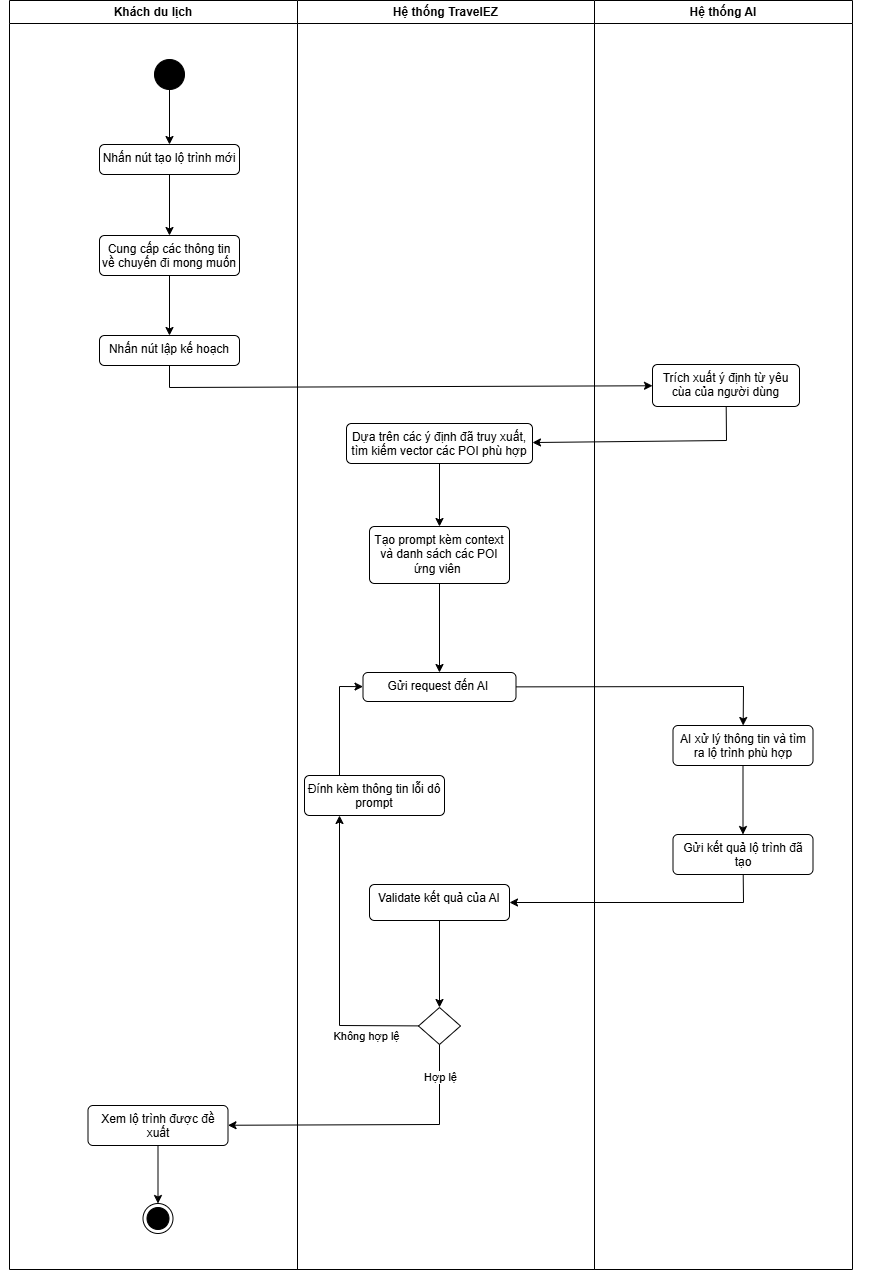
\includegraphics[width=0.9\textwidth]{Images/6. System analysis/act_m1_itinerary_recommendation.png}
    \caption{Activity diagram: Quy trình gợi ý lộ trình cá nhân hóa}
    \label{fig:activity_tao_lo_trinh}
\end{figure}

% --- QUY TRÌNH 2: Quy trình Kiểm duyệt Nội dung Tự động ---
\begin{figure}[H]
    \centering
    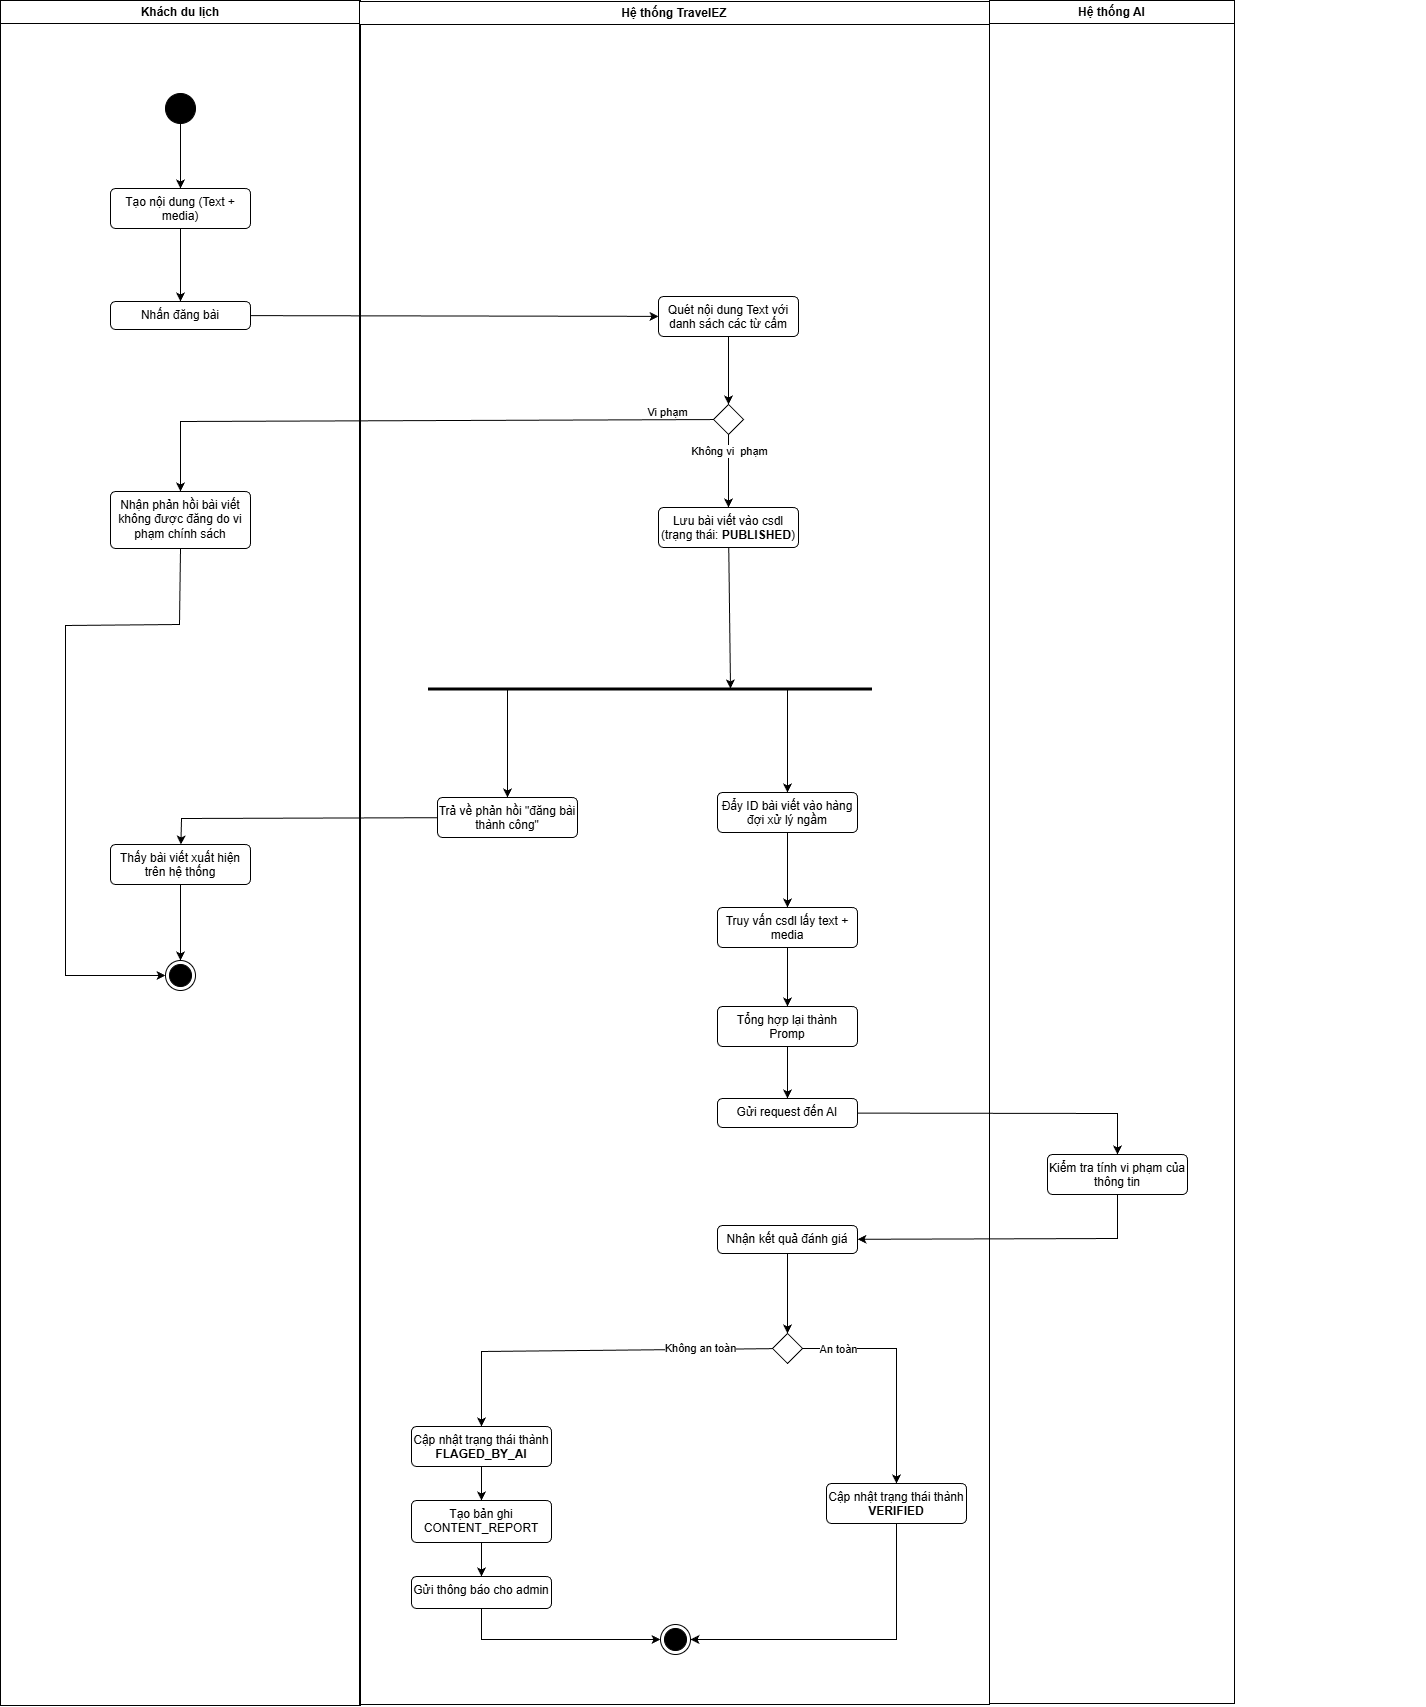
\includegraphics[width=0.9\textwidth]{Images/6. System analysis/act_m5_content_moderation.png}
    \caption{Activity diagram: Quy trình Kiểm duyệt Nội dung Tự động}
    \label{fig:activity_kiem_duyet_noi_dung}
\end{figure}

% --- QUY TRÌNH 3: PHÂN TÍCH XU HƯỚNG THỊ TRƯỜNG ---
\begin{figure}[H]
    \centering
    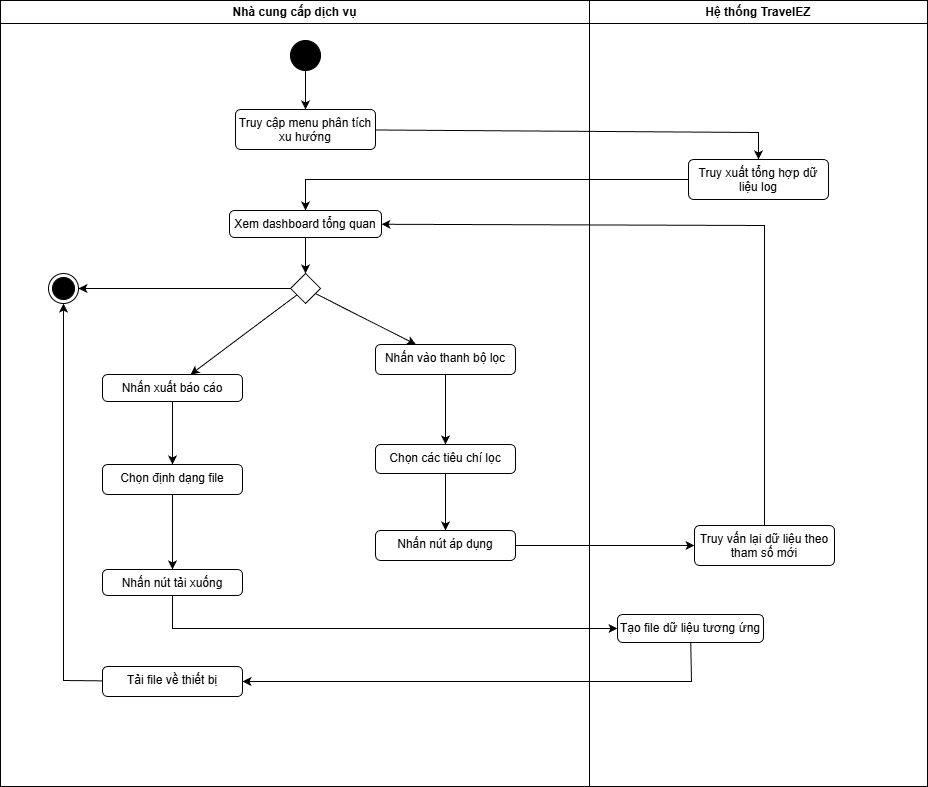
\includegraphics[width=0.9\textwidth]{Images/6. System analysis/act_m6_market_trend_analysis.png}
    \caption{Activity diagram: Quy trình phân tích xu hướng thị trường}
    \label{fig:activity_phan_tich_thi_truong}
\end{figure}

% --- QUY TRÌNH 4: PHÂN TÍCH LỊCH TRÌNH CẢI THIỆN ---
\begin{figure}[H]
    \centering
    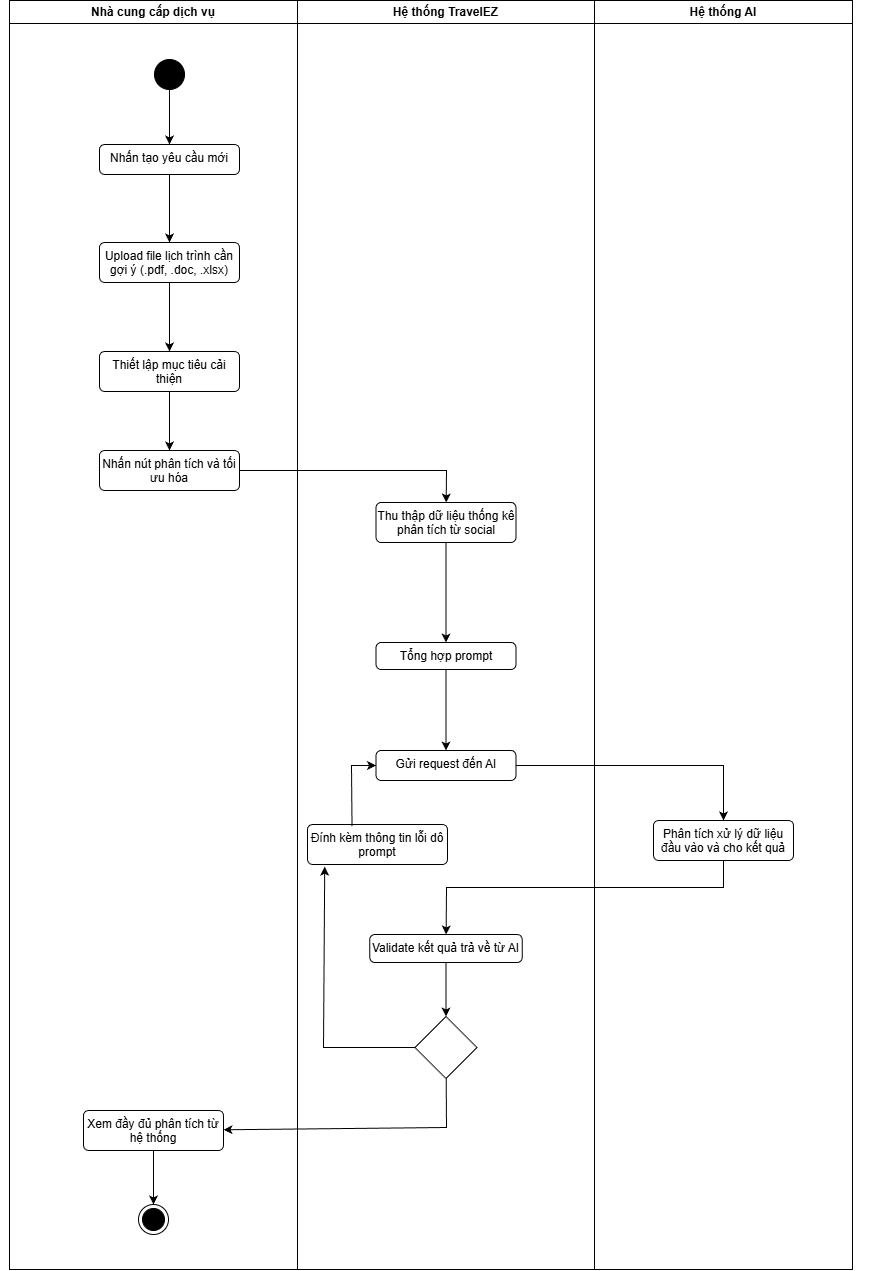
\includegraphics[width=0.9\textwidth]{Images/6. System analysis/act_m7_itinerary_optimization.png}
    \caption{Activity diagram: Quy trình phân tích lịch trình cải thiện}
    \label{fig:activity_phan_tich_lich_trinh}
\end{figure}

\subsubsection{Mô hình hoá tương tác}

% --- 1. BIỂU ĐỒ TỔNG QUAN ---
\begin{figure}[H]
    \centering
    % NOTE: Đây là file ảnh tổng quan bạn đã có
    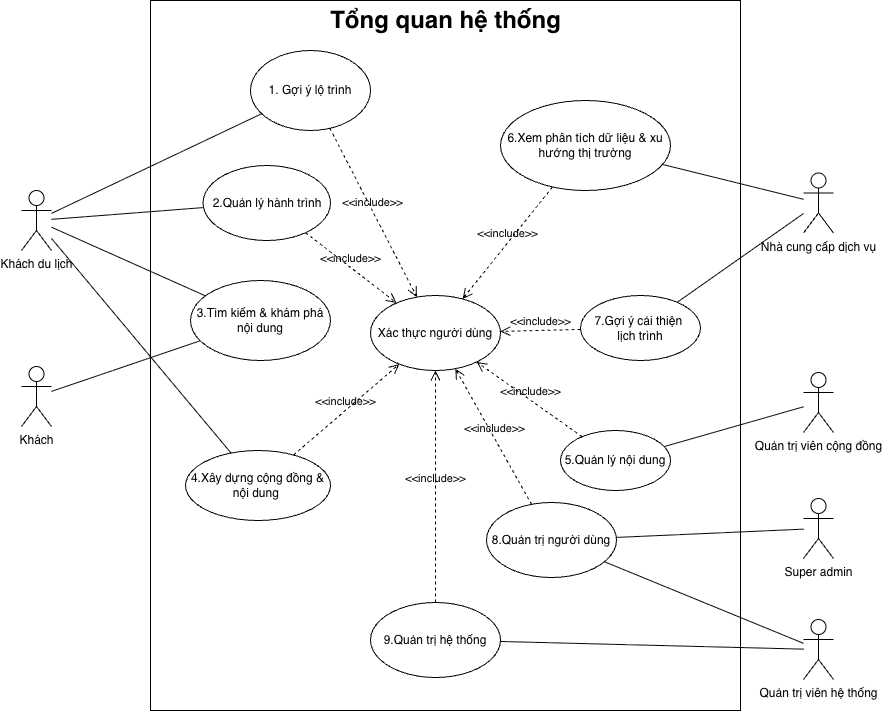
\includegraphics[width=0.9\textwidth]{Images/6. System analysis/0.png}
    \caption{Use case diagram cho tổng quan hệ thống}
    \label{fig:use_case_tong_quan}
\end{figure}

% --- 2. MODULE 1: GỢI Ý LỘ TRÌNH ---
\subsubsubsection{Module 1: Gợi ý lộ trình}
\begin{figure}[H]
    \centering
    % NOTE: Bổ sung tên file ảnh cho Module 1 (Gợi ý lộ trình)
    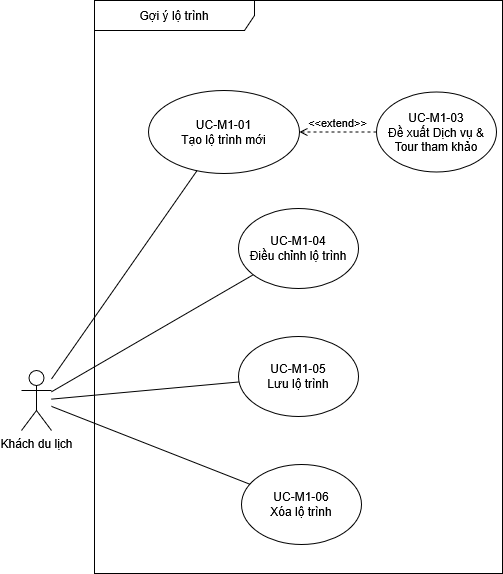
\includegraphics[width=0.9\textwidth]{Images/6. System analysis/1.png}
    \caption{Use case diagram cho Module 1: Gợi ý lộ trình}
    \label{fig:use_case_module_1}
\end{figure}
% % --- //////////////////////////////////////////////////////////////// ---
% % MODULE 1

% \renewcommand{\arraystretch}{1.2}
% \begin{longtable}{|p{4cm}|p{11cm}|}
% \caption{Mô tả Use Case: Tạo lộ trình}
% \label{usecase-1-01} \\
% \hline
% \endfirsthead
% \caption[]{Mô tả Use Case: Tạo lộ trình} \\
% \hline
% \endhead
% \textbf{Use case ID}       & UC-M1-01 \\ \hline
% \textbf{Tên Use case}      & Tạo lộ trình \\ \hline
% \textbf{Các tác nhân}      & Traveler \\ \hline
% \textbf{Mô tả}             & Traveler nhập các thông tin mong muốn cho chuyến đi (địa điểm, thời gian, ngân sách, sở thích...). Hệ thống AI tiếp nhận, phân tích và tự động tạo ra một bản lộ trình du lịch chi tiết phù hợp nhất. \\ \hline
% \textbf{Tiền điều kiện}    & Traveler đã đăng nhập và đang ở màn hình "Tạo lộ trình" \space (Dashboard hoặc Home). \\ \hline
% \textbf{Hậu điều kiện}     & Một bản nháp lộ trình hoàn chỉnh được hiển thị trên màn hình, bao gồm danh sách địa điểm và thời gian cụ thể.\\ \hline
% \textbf{Luồng sự kiện chính} & 
% \begin{tabular}[t]{@{}p{10.5cm}@{}}
% 1. Traveler nhấn nút "Tạo lộ trình mới" \space trên giao diện.\\
% 2. Hệ thống hiển thị biểu mẫu yêu cầu nhập thông tin đầu vào.\\
% 3. Traveler cung cấp các thông tin:\\
% - Điểm đến\\
% - Ngày bắt đầu và Ngày kết thúc (hoặc số ngày dự kiến)\\
% - Số lượng người tham gia (Solo, Couple, Family, Group).\\
% - Ngân sách dự kiến (Tiết kiệm, Trung bình, Sang trọng).\\
% - Sở thích/Mong muốn (Văn hóa, Ẩm thực, Mạo hiểm, Nghỉ dưỡng...).\\
% - Các lưu ý đặc biệt (Có trẻ em, Thú cưng, Cần hỗ trợ xe lăn...).\\
% 4. Traveler nhấn nút "Lập kế hoạch".\\
% 5. Hệ thống kiểm tra tính hợp lệ của dữ liệu đầu vào.\\
% 6. Hệ thống gửi dữ liệu đến Module AI xử lý.\\
% 7. AI truy xuất cơ sở dữ liệu địa điểm, tính toán khoảng cách, thời gian mở cửa và chi phí để sắp xếp lịch trình.\\
% 8. Hệ thống hiển thị bản lộ trình nháp (Timeline view) cho Traveler xem.
% \end{tabular} \\ \hline
% \textbf{Luồng rẽ nhánh A} &
% \begin{tabular}[t]{@{}p{10.5cm}@{}}
% \textbf{A1: Traveler bỏ qua các bước tùy chọn:}\\
% Tại bước 4, Traveler không chọn ngân sách hoặc sở thích. Hệ thống sẽ sử dụng giá trị mặc định (Ví dụ: Ngân sách trung bình, Sở thích phổ thông) để tạo lộ trình.\\
% \textbf{A2: Hủy tạo lộ trình:}\\
% Tại bất kỳ bước nào trước bước 4, Traveler nhấn "Hủy". Hệ thống quay lại màn hình chính.
% \end{tabular} \\ \hline
% \textbf{Luồng rẽ nhánh B: Tạo từ lộ trình có sẵn } &
% \begin{tabular}[t]{@{}p{10.5cm}@{}}
% 1. Traveler đang xem danh sách lộ trình đã đi (Lịch sử) hoặc lộ trình được chia sẻ từ bạn bè/cộng đồng.\\
% 2. Traveler chọn một lộ trình ưng ý và nhấn nút "Tạo chuyến đi từ lộ trình này" \space (hoặc "Nhân bản").\\
% 3. Hệ thống hiển thị hộp thoại yêu cầu cập nhật thông tin cơ bản:\\
% - Thời gian khởi hành mới \\
% - Tên chuyến đi mới (Mặc định là "Copy of [Tên lộ trình cũ]").\\
% 4. Traveler nhập ngày mới và nhấn "Xác nhận".\\
% 5. Hệ thống thực hiện sao chép toàn bộ danh sách địa điểm và thứ tự tham quan sang một bản ghi mới.\\
% - Lưu ý: Hệ thống tự động kiểm tra địa điểm (lịch hoạt động) và tính toán lại ngày/giờ cụ thể dựa trên ngày khởi hành mới.\\
% 6. Hệ thống chuyển hướng Traveler đến màn hình chi tiết lộ trình mới tạo để tiếp tục chỉnh sửa (kết nối sang UC-M1-04).
% \end{tabular} \\ \hline
% \textbf{Luồng ngoại lệ} &
% \begin{tabular}[t]{@{}p{10.5cm}@{}}
% \textbf{E1: Dữ liệu nhập không hợp lệ:}\\
% Tại bước 5, hệ thống phát hiện Ngày kết thúc nhỏ hơn Ngày bắt đầu hoặc Địa điểm không tồn tại. Hệ thống hiển thị thông báo lỗi ngay tại trường nhập liệu và yêu cầu nhập lại.\\
% \textbf{E2: Không tìm thấy lộ trình phù hợp:}\\
% Tại bước 8, AI không tìm thấy đủ địa điểm thỏa mãn các ràng buộc quá khắt khe của Traveler (ví dụ: Ngân sách quá thấp cho địa điểm sang trọng). Hệ thống hiển thị thông báo: "Không thể tạo lộ trình với các tiêu chí hiện tại. Vui lòng nới lỏng các yêu cầu về ngân sách hoặc thời gian."\\
% \textbf{E3: Lỗi kết nối Server:}\\
% Hệ thống thông báo "Đã xảy ra lỗi kết nối, vui lòng thử lại sau."\\
% \textbf{E4: Lộ trình gốc bị lỗi/xóa:}\\
% Khi nhấn "Nhân bản", hệ thống phát hiện lộ trình gốc đã bị xóa hoặc không còn quyền truy cập. Hiển thị thông báo: "Không thể sao chép lộ trình này."
% \end{tabular} \\ 
% \hline
% \end{longtable}

% % \renewcommand{\arraystretch}{1.2}
% % \begin{longtable}{|p{4cm}|p{11cm}|}
% % \caption{Mô tả Use Case: Đề xuất Dịch vụ \& Tour tham khảo}
% % \label{usecase-1-03} \\
% % \hline
% % \endfirsthead
% % \caption[]{Mô tả Use Case: Đề xuất Dịch vụ \& Tour tham khảo} \\
% % \hline
% % \endhead
% % \textbf{Use case ID}       & UC-M1-03 \\ \hline
% % \textbf{Tên Use case}      & Đề xuất Dịch vụ \& Tour tham khảo \\ \hline
% % \textbf{Các tác nhân}      & Traveler \\ \hline
% % \textbf{Mô tả}             & Dựa trên địa điểm hoặc khu vực mà Traveler đang xem trong lộ trình, hệ thống phân tích và đề xuất các dịch vụ thương mại phù hợp (Tour trọn gói, vé tham quan, hoặc phương tiện di chuyển du lịch) giúp người dùng dễ dàng đặt chỗ. \\ \hline
% % \textbf{Tiền điều kiện}    & Traveler đã đăng nhập vào hệ thống và đang xem một lộ trình chi tiết có chứa các địa điểm hoặc hoạt động cụ thể.\\ \hline
% % \textbf{Hậu điều kiện}     & Hệ thống đề xuất các dịch vụ phù hợp với địa điểm \\ \hline
% % \textbf{Luồng sự kiện chính} &
% % \begin{tabular}[t]{@{}p{10.5cm}@{}}
% % 1. Traveler chọn một địa điểm hoặc một khu vực trong lộ trình chi tiết.\\
% % 2. Traveler nhấn nút "Gợi ý dịch vụ/Tour".\\
% % 3. Hệ thống nhận diện Loại địa điểm và Tags của địa điểm được chọn.\\
% % 4. Hệ thống áp dụng Quy tắc gợi ý (Recommendation Rules) để lọc các dịch vụ liên kết trong CSDL:\\
% % - Kiểm tra xem địa điểm có yêu cầu vé vào cửa không.\\
% % - Kiểm tra xem địa điểm có nằm xa trung tâm và thường cần tour dẫn đường không.\\
% % - Kiểm tra xem địa điểm có phải là một thành phố lớn phù hợp với City Tour không.\\
% % 5. Hệ thống truy xuất danh sách dịch vụ của các đối tác trong CSDL phân loại rõ ràng (Vé, Tour ngày, Di chuyển).\\
% % 6. Hệ thống hiển thị danh sách đề xuất dạng thẻ kèm giá.
% % \end{tabular} \\ \hline
% % \textbf{Luồng ngoại lệ} &
% % \begin{tabular}[t]{@{}p{10.5cm}@{}}
% % \textbf{E1: Không tìm thấy thông tin:}\\
% % Tại bước 5 hoặc 6, hệ thống không tìm thấy thông tin dịch vụ liên quan nào trong CSDL, Hệ thống hiển thị thông báo "Không tìm thấy thông tin dịch vụ cho mục này."
% % \end{tabular} \\
% % \hline
% % \end{longtable}

% % \renewcommand{\arraystretch}{1.2}
% % \begin{longtable}{|p{4cm}|p{11cm}|}
% % \caption{Mô tả Use Case: Điều chỉnh lộ trình}
% % \label{usecase-1-04} \\
% % \hline
% % \endfirsthead
% % \caption[]{Mô tả Use Case: Điều chỉnh lộ trình} \\
% % \hline
% % \endhead
% % \textbf{Use case ID}       & UC-M1-04 \\ \hline
% % \textbf{Tên Use case}      & Điều chỉnh lộ trình \\ \hline
% % \textbf{Các tác nhân}      & Traveler \\ \hline
% % \textbf{Mô tả}             & Traveler thực hiện tinh chỉnh lộ trình theo ý muốn cá nhân hoặc đưa ra yêu cầu để AI tái cấu trúc lại một phần hoặc toàn bộ lộ trình dựa trên ngữ cảnh mới.\\ \hline
% % \textbf{Tiền điều kiện}    & 
% % \begin{tabular}[t]{@{}p{10.5cm}@{}}
% % 1. Traveler đang xem chi tiết một bản lộ trình (nháp hoặc đã lưu).\\
% % 2. Lộ trình đang ở trạng thái có thể chỉnh sửa (không phải lộ trình của người khác chia sẻ dạng view-only).
% % \end{tabular} \\ \hline
% % \textbf{Hậu điều kiện}     & Lộ trình được cập nhật với thứ tự, thời gian và địa điểm mới hợp lý. Dữ liệu được lưu lại. \\ \hline
% % \textbf{Luồng sự kiện chính} &
% % \begin{tabular}[t]{@{}p{10.5cm}@{}}
% % 1. Traveler chọn một hoạt động/địa điểm trong lộ trình.\\
% % 2. Traveler thực hiện thao tác chỉnh sửa thủ công:
% % - Kéo thả (Drag \& drop) để đổi thứ tự tham quan.\\
% % - Thay đổi thời gian bắt đầu/kết thúc thủ công.\\
% % - Xóa một địa điểm khỏi lịch trình.\\
% % 3. Hệ thống tự động tính toán lại thời gian di chuyển giữa các điểm liền kề.\\
% % 4. Hệ thống kiểm tra xung đột logic cơ bản (ví dụ: trùng giờ, điểm đến đóng cửa vào giờ mới chọn).\\
% % 5. Nếu có xung đột, hệ thống hiển thị cảnh báo (Warning flag) nhưng vẫn cho phép Traveler giữ nguyên nếu muốn.\\
% % 6. Traveler nhấn "Lưu thay đổi".
% % \end{tabular} \\ \hline
% % \textbf{Luồng rẽ nhánh A: AI sửa đổi theo yêu cầu }    & 
% % \begin{tabular}[t]{@{}p{10.5cm}@{}}
% % 1. Traveler xem lộ trình, xác định các điểm "cứng" \space (Check-in khách sạn, Giờ bay, Bữa tối đặt bàn).\\
% % 2. Traveler nhấn icon Pin (Ghim) vào các điểm đó.\\
% % 3. Traveler nhấn "Tối ưu đường đi".\\
% % 4. Hệ thống hiển thị các tùy chọn sửa đổi:\\
% % - Tối ưu đường đi: Giữ nguyên địa điểm, chỉ sắp xếp lại thứ tự cho thuận tiện nhất.\\
% % - Thay đổi nhịp độ: "Lịch trình quá dày, hãy làm giãn ra" \space hoặc "Thêm địa điểm vào chỗ trống".\\
% % - Thay đổi chủ đề: "Đổi ngày 2 sang food tour thay vì tham quan bảo tàng".\\
% % 5. Hệ thống tính toán và sắp xếp lại thứ tự các điểm chưa ghim.
% % \end{tabular} \\ \hline
% % \textbf{Luồng rẽ nhánh B: Thay thế một địa điểm cụ thể}    & 
% % \begin{tabular}[t]{@{}p{10.5cm}@{}}
% % 1. Traveler không thích một địa điểm cụ thể.\\
% % 2. Traveler chọn địa điểm đó và nhấn "Gợi ý thay thế".\\
% % 3. Hệ thống tìm kiếm các địa điểm lân cận có cùng tính chất hoặc phù hợp với sở thích của Traveler.\\
% % 4. Hệ thống hiển thị danh sách 3-5 địa điểm thay thế.\\
% % 5. Traveler chọn 1 địa điểm mới.\\
% % 6. Hệ thống thế chỗ địa điểm cũ bằng địa điểm mới và cập nhật lại thời gian/chi phí.    
% % \end{tabular} \\ \hline
% % \textbf{Luồng ngoại lệ} &
% % \begin{tabular}[t]{@{}p{10.5cm}@{}}
% % \textbf{E1: Yêu cầu AI bất khả thi:}\\
% % Traveler yêu cầu "Thêm 5 địa điểm" \space vào một ngày đã kín lịch. AI thông báo: "Không đủ thời gian để thêm địa điểm. Bạn có muốn mở rộng chuyến đi thêm 1 ngày không?"\\
% % \textbf{E2: Xung đột giờ mở cửa:}\\
% % Khi kéo thả thủ công, Traveler đặt một địa điểm vào khung giờ nó đóng cửa. Hệ thống hiện cảnh báo đỏ: "Địa điểm này đóng cửa lúc 17:00."
% % \end{tabular} \\
% % \hline
% % \end{longtable}

% % \renewcommand{\arraystretch}{1.2}
% % \begin{longtable}{|p{4cm}|p{11cm}|}
% % \caption{Mô tả Use Case: Lưu Lộ trình}
% % \label{usecase-1-05} \\
% % \hline
% % \endfirsthead
% % \caption[]{Mô tả Use Case: Lưu Lộ trình} \\
% % \hline
% % \endhead
% % \textbf{Use case ID}       & UC-M1-05 \\ \hline
% % \textbf{Tên Use case}      & Lưu Lộ trình \\ \hline
% % \textbf{Các tác nhân}      & Traveler \\ \hline
% % \textbf{Mô tả}             & Lưu trạng thái hiện tại của lộ trình vào tài khoản cá nhân để truy cập sau.\\ \hline
% % \textbf{Tiền điều kiện}    & Traveler đã đăng nhập và đang có một lộ trình trên màn hình. \\ \hline
% % \textbf{Hậu điều kiện}     & Dữ liệu lộ trình được ghi vào CSDL. \\ \hline
% % \textbf{Luồng sự kiện chính} &
% % \begin{tabular}[t]{@{}p{10.5cm}@{}}
% % 1. Traveler nhấn nút "Lưu lộ trình".\\
% % 2. Hệ thống kiểm tra trạng thái lộ trình:\\
% % - Trường hợp A (Lộ trình mới): Hệ thống hiển thị Popup yêu cầu nhập "Tên chuyến đi".\\
% % - Trường hợp B (Lộ trình đã tồn tại): Hệ thống bỏ qua bước 3.\\
% % 3. (Nếu là mới) Traveler nhập tên và nhấn "Xác nhận".\\
% % 4. Hệ thống thu thập toàn bộ dữ liệu (JSON/XML cấu trúc chuyến đi).\\
% % 5. Hệ thống lưu vào cơ sở dữ liệu.\\
% % 6. Hệ thống thông báo "Đã lưu thành công".
% % \end{tabular} \\ \hline
% % \textbf{Luồng ngoại lệ} &
% % \begin{tabular}[t]{@{}p{10.5cm}@{}}
% % \textbf{E1: Trùng tên (Khi lưu mới):}\\
% % Traveler nhập tên đã có trong danh sách của mình. Hệ thống báo lỗi và yêu cầu chọn tên khác.\\
% % \textbf{E2: Lỗi hệ thống:}\\
% % Lưu thất bại do lỗi CSDL. Thông báo lỗi và giữ nguyên màn hình để Traveler thử lại.
% % \end{tabular} \\
% % \hline
% % \end{longtable}

% % \renewcommand{\arraystretch}{1.2}
% % \begin{longtable}{|p{4cm}|p{11cm}|}
% % \caption{Mô tả Use Case: Xóa Lộ trình}
% % \label{usecase-1-06} \\
% % \hline
% % \endfirsthead
% % \caption[]{Mô tả Use Case: Xóa Lộ trình} \\
% % \hline
% % \endhead
% % \textbf{Use case ID}       & UC-M1-06 \\ \hline
% % \textbf{Tên Use case}      & Xóa Lộ trình \\ \hline
% % \textbf{Các tác nhân}      & Traveler \\ \hline
% % \textbf{Mô tả}             & Xóa vĩnh viễn một lộ trình đã lưu khỏi tài khoản. \\ \hline
% % \textbf{Tiền điều kiện}    & Traveler đang ở màn hình danh sách lộ trình ("Chuyến đi của tôi"). \\ \hline
% % \textbf{Hậu điều kiện}     & Lộ trình bị loại bỏ khỏi CSDL và không còn hiển thị trong danh sách. \\ \hline
% % \textbf{Luồng sự kiện chính} &
% % \begin{tabular}[t]{@{}p{10.5cm}@{}}
% % 1. Traveler chọn lộ trình muốn xóa từ danh sách.\\
% % 2. Traveler nhấn nút "Xóa" \space (icon thùng rác).\\
% % 3. Hệ thống hiển thị hộp thoại xác nhận: "Bạn có chắc chắn muốn xóa lộ trình này? Hành động này không thể hoàn tác."\\
% % 4. Traveler nhấn "Đồng ý" \space (Confirm).\\
% % 5. Hệ thống gửi lệnh xóa xuống CSDL.\\
% % 6. Hệ thống cập nhật lại danh sách hiển thị (biến mất dòng tương ứng).\\
% % 7. Hệ thống thông báo "Đã xóa thành công".    
% % \end{tabular} \\ \hline
% % \textbf{Luồng rẽ nhánh}    & 
% % \begin{tabular}[t]{@{}p{10.5cm}@{}}
% % \textbf{A1: Hủy xóa:}\\
% % Tại bước 3, Traveler nhấn "Hủy". Hộp thoại đóng lại, không có gì thay đổi.
% % \end{tabular} \\
% % \hline
% % \end{longtable}


% --- 3. MODULE 2: QUẢN LÝ LỘ TRÌNH ---
\subsubsubsection{Module 2: Quản lý lộ trình}
\begin{figure}[H]
    \centering
    % NOTE: Bổ sung tên file ảnh cho Module 2 (Quản lý lộ trình)
    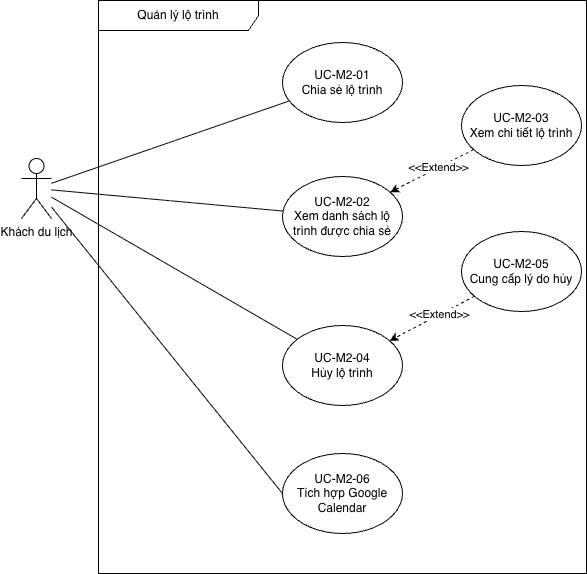
\includegraphics[width=0.9\textwidth]{Images/6. System analysis/2.png}
    \caption{Use case diagram cho Module 2: Quản lý lộ trình}
    \label{fig:use_case_module_2}
\end{figure}
% --- //////////////////////////////////////////////////////////////// ---
% MODULE 2
\begin{longtable}{@{}p{4cm} p{11cm}@{}}
\caption{Mô tả Use Case: Chia sẻ Lộ trình}
\label{usecase-2-01} \\
\toprule
\textbf{Use case ID}       & UC-M2-01 \\ \midrule
\textbf{Tên Use case}      & Chia sẻ Lộ trình \\ \midrule
\textbf{Các tác nhân}      & Traveler \\ \midrule
\textbf{Mô tả}             & Cho phép Traveler chia sẻ một lộ trình đã lưu của mình cho một hoặc nhiều Traveler khác. Những người được chia sẻ chỉ có quyền xem nội dung lộ trình. \\ \midrule
\textbf{Tiền điều kiện}    & 
\begin{tabular}[t]{@{}p{10.5cm}@{}}
1. Traveler đã đăng nhập vào hệ thống.\\
2. Lộ trình muốn chia sẻ đã được lưu vào tài khoản.
\end{tabular} \\ \midrule
\textbf{Hậu điều kiện}     & Quyền xem lộ trình được cấp thành công cho các Traveler được chỉ định. \\ \midrule
\textbf{Luồng sự kiện chính} & 
\begin{tabular}[t]{@{}p{10.5cm}@{}}
1. Traveler mở một lộ trình đã lưu và nhấn vào nút ""Chia sẻ"".\\
2. Hệ thống hiển thị một giao diện, bao gồm một ô nhập liệu để tìm kiếm người dùng.\\
3. Traveler nhập tên tài khoản của người mà họ muốn chia sẻ. Hệ thống có thể hiển thị các gợi ý tìm kiếm.\\
4. Traveler chọn một hoặc nhiều tài khoản từ kết quả tìm kiếm.\\
5. Traveler nhấn nút ""Xác nhận chia sẻ"".\\
6. Hệ thống kiểm tra sự tồn tại và hợp lệ của các tài khoản được chọn.\\
7. Hệ thống tạo một bản ghi về quyền truy cập trong cơ sở dữ liệu, cấp quyền ""chỉ xem"" cho các tài khoản được chọn đối với lộ trình này.\\
8. Hệ thống hiển thị thông báo ""Đã chia sẻ lộ trình thành công!""
\end{tabular} \\ \midrule
\textbf{Luồng rẽ nhánh}    & N/A \\ \midrule
\textbf{Luồng ngoại lệ} &
\begin{tabular}[t]{@{}p{10.5cm}@{}}
\textbf{E1: Không tìm thấy tài khoản người dùng:}\\
Thời điểm: Xảy ra tại bước 3.\\
Mô tả: Traveler nhập một tên tài khoản không tồn tại trong hệ thống. Hệ thống sẽ hiển thị thông báo ""Không tìm thấy người dùng này.""\\[3pt]
\textbf{E2: Lỗi hệ thống khi cấp quyền}\\
Thời điểm: Xảy ra tại bước 7.\\
Mô tả: Hệ thống không thể lưu lại quyền chia sẻ do lỗi kết nối hoặc lỗi máy chủ. Hệ thống sẽ hiển thị thông báo ""Chia sẻ thất bại, vui lòng thử lại.""
\end{tabular} \\ 
\bottomrule
\end{longtable}

\begin{longtable}{@{}p{4cm} p{11cm}@{}}
\caption{Mô tả Use Case: Xem Lộ trình được chia sẻ}
\label{usecase-2-02} \\
\toprule
\textbf{Use case ID}       & UC-M2-02 \\ \midrule
\textbf{Tên Use case}      & Xem Lộ trình được chia sẻ \\ \midrule
\textbf{Các tác nhân}      & Traveler \\ \midrule
\textbf{Mô tả}             & Cho phép Traveler xem danh sách các lộ trình mà những người dùng khác đã chia sẻ cho họ, và mở ra để xem chi tiết. \\ \midrule
\textbf{Tiền điều kiện}    & 
\begin{tabular}[t]{@{}p{10.5cm}@{}}
1. Traveler đã đăng nhập vào hệ thống.\\
2. Có ít nhất một Traveler khác đã chia sẻ lộ trình cho họ.
\end{tabular} \\ \midrule
\textbf{Hậu điều kiện}     & Traveler xem được nội dung chi tiết của lộ trình đã được chia sẻ. \\ \midrule
\textbf{Luồng sự kiện chính} &
\begin{tabular}[t]{@{}p{10.5cm}@{}}
1. Traveler truy cập vào trang quản lý hành trình cá nhân.\\
2. Họ chọn vào mục hoặc tab ""Được chia sẻ với tôi"".\\
3. Hệ thống truy vấn và hiển thị một danh sách các lộ trình mà Traveler này đã được cấp quyền xem, có thể kèm theo tên người chia sẻ.\\
4. Traveler nhấn vào một lộ trình trong danh sách.\\
5. Hệ thống hiển thị nội dung chi tiết của lộ trình đó ở chế độ chỉ xem (view-only). Tất cả các nút chỉnh sửa, xóa đều bị ẩn hoặc vô hiệu hóa.
\end{tabular} \\ \midrule
\textbf{Luồng rẽ nhánh}    & N/A \\ \midrule
\textbf{Luồng ngoại lệ} &
\begin{tabular}[t]{@{}p{10.5cm}@{}}
\textbf{E1: Người chia sẻ đã thu hồi quyền truy cập:}\\
Thời điểm: Xảy ra tại bước 4.\\
Mô tả: Traveler nhấn vào một lộ trình nhưng người chia sẻ đã hủy quyền truy cập trước đó. Hệ thống sẽ hiển thị thông báo ""Bạn không còn quyền truy cập vào lộ trình này.""\\[3pt]
\textbf{E2: Lộ trình gốc đã bị xóa:}\\
Thời điểm: Xảy ra tại bước 4.\\
Mô tả: Lộ trình mà người dùng muốn xem đã bị người tạo ra xóa vĩnh viễn. Hệ thống sẽ hiển thị thông báo ""Lộ trình này không còn tồn tại.""
\end{tabular} \\
\bottomrule
\end{longtable}

\begin{longtable}{@{}p{4cm} p{11cm}@{}}
\caption{Mô tả Use Case: Hủy Lộ trình}
\label{usecase-2-04} \\
\toprule
\textbf{Use case ID}       & UC-M2-04 \\ \midrule
\textbf{Tên Use case}      & Hủy Lộ trình \\ \midrule
\textbf{Các tác nhân}      & Traveler \\ \midrule
\textbf{Mô tả}             & Cho phép Traveler thay đổi trạng thái của một lộ trình từ ""Đang tiến hành"" sang ""Đã hủy"". Traveler sẽ được yêu cầu cung cấp lý do cho việc hủy. \\ \midrule
\textbf{Tiền điều kiện}    & 
\begin{tabular}[t]{@{}p{10.5cm}@{}}
1. Traveler đã đăng nhập.\\
2. Traveler có một lộ trình đang ở trạng thái ""Đang tiến hành""
\end{tabular} \\ \midrule
\textbf{Hậu điều kiện}     & Trạng thái của lộ trình được chuyển thành ""Đã hủy"". Lý do hủy (nếu có) được ghi nhận. \\ \midrule
\textbf{Luồng sự kiện chính} &
\begin{tabular}[t]{@{}p{10.5cm}@{}}
1. Vào ngày bắt đầu của lộ trình, hệ thống tự động chuyển trạng thái thành ""Đang tiến hành"".\\
2. Giao diện người dùng hiển thị lộ trình này kèm theo nút ""Hủy Lộ trình"".\\
3. Traveler nhấn vào nút ""Hủy Lộ trình"".\\
4. Hệ thống hiển thị một hộp thoại, yêu cầu người dùng nhập lý do hủy (có thể là một ô văn bản hoặc chọn từ danh sách có sẵn).\\
5. Traveler nhập lý do và nhấn ""Xác nhận hủy"".\\
6. Hệ thống cập nhật trạng thái của lộ trình trong cơ sở dữ liệu thành ""Đã hủy"".\\
7. Hệ thống lưu lại lý do mà người dùng đã cung cấp (phục vụ cho mục đích thống kê sau này).\\
8. Giao diện hiển thị thông báo ""Lộ trình đã được hủy"".
\end{tabular} \\ \midrule
\textbf{Luồng rẽ nhánh}    &
\begin{tabular}[t]{@{}p{10.5cm}@{}}
\textbf{A1: Hủy không cần lý do:}\\
Thời điểm: Xảy ra tại bước 5, nếu việc nhập lý do là không bắt buộc.\\
Mô tả: Traveler có thể bỏ qua việc nhập lý do và nhấn ""Xác nhận hủy"" trực tiếp. Luồng tiếp tục bình thường.
\end{tabular} \\ \midrule
\textbf{Luồng ngoại lệ} &
\begin{tabular}[t]{@{}p{10.5cm}@{}}
\textbf{E1: Lỗi kết nối hoặc lỗi máy chủ:}\\
Thời điểm: Xảy ra tại bước 6.\\
Mô tả: Hệ thống không thể cập nhật trạng thái do lỗi. Hệ thống sẽ hiển thị thông báo ""Hủy thất bại, vui lòng thử lại.""
\end{tabular} \\
\bottomrule
\end{longtable}

\begin{longtable}{@{}p{4cm} p{11cm}@{}}
\caption{Mô tả Use Case: Tích hợp Lộ trình với Google Calendar}
\label{usecase-2-06} \\
\toprule
\textbf{Use case ID}       & UC-M2-06 \\ \midrule
\textbf{Tên Use case}      & Tích hợp Lộ trình với Google Calendar \\ \midrule
\textbf{Các tác nhân}      & Traveler (Primary), Google Calendar (Secondary) \\ \midrule
\textbf{Mô tả}             & Cho phép Traveler đồng bộ (xuất) một lộ trình đã lưu của họ sang tài khoản Google Calendar cá nhân để tiện theo dõi lịch trình trên các thiết bị khác. \\ \midrule
\textbf{Tiền điều kiện}    & 
\begin{tabular}[t]{@{}p{10.5cm}@{}}
1. Traveler đã đăng nhập vào hệ thống.\\
2. Traveler có ít nhất một lộ trình đã lưu (có thông tin ngày, giờ cụ thể).\\
3. Traveler đang xem chi tiết lộ trình mà họ muốn đồng bộ.
\end{tabular} \\ \midrule
\textbf{Hậu điều kiện}     & 
\begin{tabular}[t]{@{}p{10.5cm}@{}}
(Thành công): Các hoạt động trong lộ trình được tạo thành công dưới dạng các Sự kiện (Events) trên Google Calendar của Traveler.\\
(Thất bại): Lộ trình không được đồng bộ, hệ thống hiển thị thông báo lỗi.
\end{tabular} \\ \midrule
\textbf{Luồng sự kiện chính} &
\begin{tabular}[t]{@{}p{10.5cm}@{}}
1. Traveler đang xem chi tiết một lộ trình đã lưu.\\
2. Traveler nhấn vào nút “Tích hợp Google Calendar” (hoặc “Thêm vào Lịch”).\\
3. Hệ thống chuyển hướng Traveler đến trang xác thực OAuth 2.0 của Google.\\
4. Hệ thống yêu cầu Traveler cấp quyền cho ứng dụng TravelEZ để ""Xem và quản lý lịch"" của họ.\\
5. Traveler chọn tài khoản Google và nhấn ""Cho phép"".\\
6. Google trả về mã xác thực (authorization code) cho hệ thống TravelEZ.\\
7. Hệ thống dùng mã này để lấy Access Token truy cập Google Calendar API.\\
8. Hệ thống đọc dữ liệu chi tiết của lộ trình (tên hoạt động, địa điểm, thời gian bắt đầu, thời gian kết thúc).\\
9. Hệ thống lặp qua từng hoạt động và gọi API của Google Calendar để tạo các sự kiện tương ứng.\\
10. Hệ thống hiển thị thông báo ""Đã đồng bộ lộ trình sang Google Calendar thành công!""
\end{tabular} \\ \midrule
\textbf{Luồng rẽ nhánh}    &
\begin{tabular}[t]{@{}p{10.5cm}@{}}
\textbf{A1: Người dùng đã cấp quyền trước đó:}\\
Tại bước 3, hệ thống phát hiện đã có Access Token hợp lệ của người dùng.\\
Hệ thống bỏ qua các bước 4, 5, 6, 7.\\
Luồng sự kiện tiếp tục từ bước 8.
\end{tabular} \\ \midrule
\textbf{Luồng ngoại lệ} &
\begin{tabular}[t]{@{}p{10.5cm}@{}}
\textbf{E1: Người dùng từ chối cấp quyền:}\\
Tại bước 5, Traveler nhấn ""Từ chối"" hoặc đóng cửa sổ xác thực.\\
Hệ thống hiển thị thông báo ""Không thể tích hợp nếu không được cấp quyền truy cập."" Use case kết thúc.\\[3pt]
\textbf{E2: Lỗi Google Calendar API:}\\
Tại bước 9, API của Google trả về lỗi (ví dụ: token hết hạn, API service down, không tìm thấy lịch chính...).\\
Hệ thống hiển thị thông báo ""Đã xảy ra lỗi khi đồng bộ. Vui lòng thử lại sau.""\\[3pt]
\textbf{E3: Lộ trình không có dữ liệu thời gian:}\\
Tại bước 8, hệ thống phát hiện lộ trình đang xem không có thông tin ngày/giờ cụ thể (ví dụ: chỉ là một danh sách địa điểm).\\
Hệ thống hiển thị thông báo ""Không thể đồng bộ lộ trình chưa được lập lịch. Vui lòng thêm ngày giờ cho các hoạt động."" Use case kết thúc.
\end{tabular} \\
\bottomrule
\end{longtable}


% --- 4. MODULE 3: TÌM KIẾM VÀ KHÁM PHÁ NỘI DUNG ---
\subsubsubsection{Module 3: Tìm kiếm và khám phá nội dung}
\begin{figure}[H]
    \centering
    % NOTE: Bổ sung tên file ảnh cho Module 3 (Tìm kiếm và khám phá nội dung)
    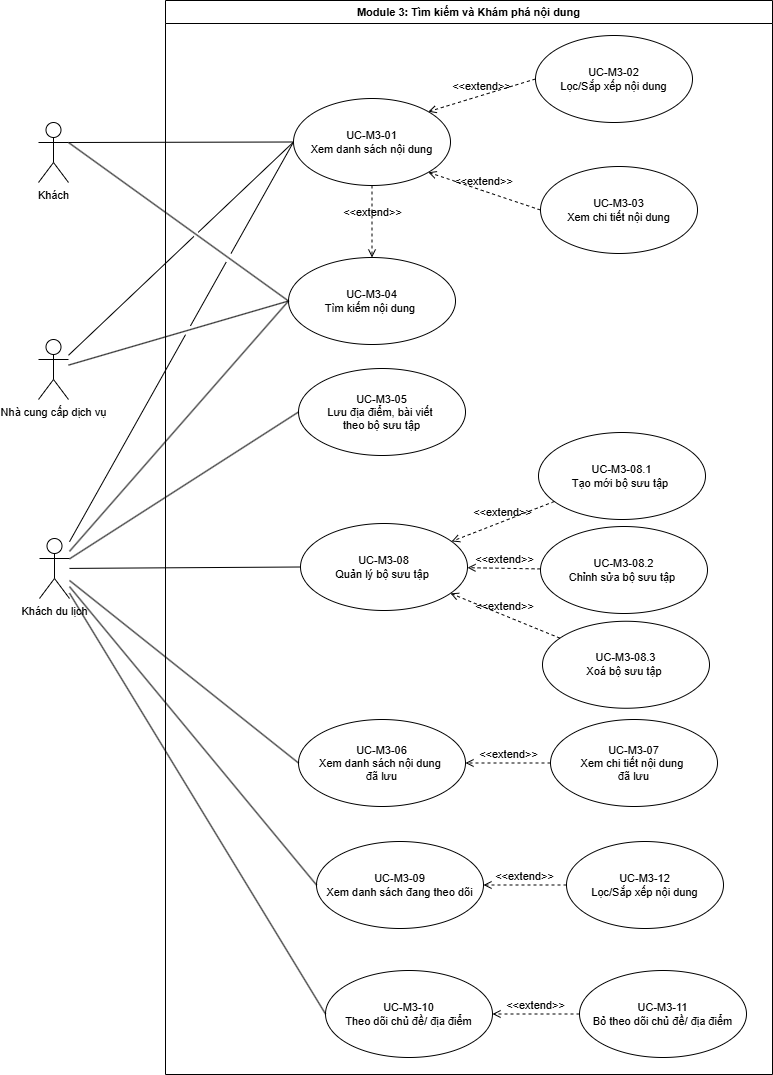
\includegraphics[width=0.9\textwidth]{Images/6. System analysis/3.png}
    \caption{Use case diagram cho Module 3: Tìm kiếm \& khám phá nội dung}
    \label{fig:use_case_module_3}
\end{figure}
\begin{table}[H]
\caption{Mô tả Use Case: Xem danh sách nội dung}
\label{usecase-3-01}
\centering
\renewcommand{\arraystretch}{1.2}
\begin{tabular}{@{}p{4cm} p{11cm}@{}}
\toprule
\textbf{Use case ID}       & UC-M3-01 \\ \midrule
\textbf{Tên Use case}      & Xem danh sách nội dung \\ \midrule
\textbf{Các tác nhân}      & Traveler, Guest, Provider \\ \midrule
\textbf{Mô tả}             & Cho phép người dùng xem danh sách bài viết hiển thị trên trang chủ hoặc bảng tin khám phá hoặc theo chủ đề. \\ \midrule
\textbf{Tiền điều kiện}    & Hệ thống đã có sẵn dữ liệu nội dung. \\ \midrule
\textbf{Hậu điều kiện}     & Danh sách nội dung được hiển thị theo bộ lọc mặc định hoặc tùy chọn người dùng. \\ \midrule
\textbf{Luồng sự kiện chính} & 
\begin{tabular}[t]{@{}p{10.5cm}@{}}
1. Người dùng truy cập trang chủ hoặc bảng tin khám phá.\\
2. Hệ thống hiển thị danh sách nội dung công khai theo thứ tự mặc định.
\end{tabular} \\ \midrule
\textbf{Luồng ngoại lệ} & 2a. Nếu hệ thống bị mất kết nối, màn hình hiển thị “Lỗi kết nối” \\ 
\bottomrule
\end{tabular}
\end{table}

\begin{table}[H]
\caption{Mô tả Use Case: Lọc và sắp xếp nội dung}
\label{usecase-3-02}
\centering
\renewcommand{\arraystretch}{1.2}
\begin{tabular}{@{}p{4cm} p{11cm}@{}}
\toprule
\textbf{Use case ID}       & UC-M3-02 \\ \midrule
\textbf{Tên Use case}      & Lọc và sắp xếp nội dung \\ \midrule
\textbf{Các tác nhân}      & Traveler, Guest, Provider \\ \midrule
\textbf{Mô tả}             & Người dùng sắp xếp danh sách theo tiêu chí như: độ phổ biến, đánh giá cao, hoặc lọc danh sách theo các tiêu chí như: xếp hạng theo đánh giá khách hàng, khu vực, các bộ lọc đặc biệt (phù hợp với gia đình, cho phép thú cưng, phù hợp với solo-trip,...) \\ \midrule
\textbf{Trigger}    & Người dùng chọn mục "Sắp xếp theo…", "Lọc nâng cao". \\ \midrule
\textbf{Tiền điều kiện}    & Hệ thống đã có sẵn dữ liệu nội dung. \\ \midrule
\textbf{Hậu điều kiện}     & Hệ thống hiển thị danh sách kết quả tìm kiếm theo phân trang. \\ \midrule
\textbf{Luồng sự kiện chính} & 
\begin{tabular}[t]{@{}p{10.5cm}@{}}
1. Người chọn các tiêu chí lọc, sắp xếp.\\
2. Người dùng nhấn nút "Áp dụng".\\
3. Hệ thống truy vấn dữ liệu và hiển thị kết quả.
\end{tabular} \\ \midrule
\textbf{Luồng ngoại lệ} & \begin{tabular}[t]{@{}p{10.5cm}@{}}
3a. Không tìm thấy kết quả → hệ thống hiển thị thông báo "Không tìm thấy nội dung phù hợp."\\
3b. Lỗi kết nối → hiển thị "Không thể tải dữ liệu, vui lòng thử lại."
\end{tabular} \\ 
\bottomrule
\end{tabular}
\end{table}


\begin{table}[H]
\caption{Mô tả Use Case: Tìm kiếm nội dung}
\label{usecase-3-04}
\centering
\renewcommand{\arraystretch}{1.2}
\begin{tabular}{@{}p{4cm} p{11cm}@{}}
\toprule
\textbf{Use case ID}       & UC-M3-04 \\ \midrule
\textbf{Tên Use case}      & Tìm kiếm nội dung \\ \midrule
\textbf{Các tác nhân}      & Traveler, Guest, Provider \\ \midrule
\textbf{Mô tả}             & Cho phép người dùng tìm kiếm bài viết, địa điểm hoặc chủ đề theo từ khóa, danh mục. \\ \midrule
\textbf{Tiền điều kiện}    & Người dùng có thể truy cập thanh tìm kiếm. \\ \midrule
\textbf{Hậu điều kiện}     & Hệ thống hiển thị danh sách kết quả tìm kiếm theo phân trang. \\ \midrule
\textbf{Luồng sự kiện chính} & 
\begin{tabular}[t]{@{}p{10.5cm}@{}}
1. Người nhập từ khóa tìm kiếm \\
2. Người dùng nhấn nút tìm kiếm \\
3. Hệ thống truy vấn dữ liệu và hiển thị kết quả.
\end{tabular} \\ \midrule
\textbf{Luồng ngoại lệ} &
\begin{tabular}[t]{@{}p{10.5cm}@{}}
3a. Không tìm thấy kết quả → hệ thống hiển thị thông báo "Không tìm thấy nội dung phù hợp với từ khóa." \\
3b. Lỗi kết nối → hiển thị "Không thể tải dữ liệu, vui lòng thử lại."
\end{tabular} \\ \midrule
\textbf{Luồng thay thế} &
\begin{tabular}[t]{@{}p{10.5cm}@{}}
1. Người chọn danh mục/chủ đề gợi ý trên thanh công cụ tìm kiếm. \\
2. Người dùng nhấn nút tìm kiếm. \\
3. Hệ thống xử lý và hiển thị kết quả. 
\end{tabular} \\ 
\bottomrule
\end{tabular}
\end{table}

\begin{table}[H]
\caption{Mô tả Use Case: Lưu địa điểm, bài viết}
\label{usecase-3-05}
\centering
\renewcommand{\arraystretch}{1.2}
\begin{tabular}{@{}p{4cm} p{11cm}@{}}
\toprule
\textbf{Use case ID}       & UC-M3-05 \\ \midrule
\textbf{Tên Use case}      & Lưu địa điểm, bài viết \\ \midrule
\textbf{Các tác nhân}      & Traveler \\ \midrule
\textbf{Mô tả}             & Cho phép người dùng (Traveler) lưu lại bài viết hoặc địa điểm yêu thích để xem lại sau. \\ \midrule
\textbf{Trigger}    & Người dùng nhấn biểu tượng “Lưu” trên bài viết hoặc địa điểm. \\ \midrule
\textbf{Tiền điều kiện}    & Người dùng đã đăng nhập. \\ \midrule
\textbf{Hậu điều kiện}     & Nội dung được thêm vào danh sách đã lưu. \\ \midrule
\textbf{Luồng sự kiện chính} & 
\begin{tabular}[t]{@{}p{10.5cm}@{}}
1. Người dùng chọn biểu tượng "Lưu" \space tại bài viết hoặc địa điểm.\\
2. Hệ thống hiển thị danh sách "Bộ sưu tập" \space của người dùng.\\
3. Người dùng tuỳ chọn "Bộ sưu tập" \space để lưu bài viết/ địa điểm.\\
4. Hệ thống ghi nhận và thêm nội dung vào danh sách đã lưu.
\end{tabular} \\ \midrule
\textbf{Luồng ngoại lệ} &
\begin{tabular}[t]{@{}p{10.5cm}@{}}
1a. Chưa đăng nhập → hiển thị "Vui lòng đăng nhập để sử dụng tính năng lưu."
\end{tabular} \\ \midrule
\textbf{Luồng thay thế} &
\begin{tabular}[t]{@{}p{10.5cm}@{}}
3(a)1.  Người dùng chọn biểu tượng "+" \space để tạo "Bộ sưu tập".\\  
2. Hệ thống tự động lưu bài viết/ địa điểm vào bộ sưu tập vừa tạo.\\
3(b)1. Hệ thống tự động lưu bài viết/địa điểm vào danh mục mặc định "Tất cả bài viết".
\end{tabular} \\ 
\bottomrule
\end{tabular}
\end{table}

\begin{table}[H]
\caption{Mô tả Use Case: Xem danh sách nội dung địa điểm, bài viết đã lưu}
\label{usecase-3-06}
\centering
\renewcommand{\arraystretch}{1.2}
\begin{tabular}{@{}p{4cm} p{11cm}@{}}
\toprule
\textbf{Use case ID}       & UC-M3-06 \\ \midrule
\textbf{Tên Use case}      & Xem danh sách nội dung địa điểm, bài viết đã lưu \\ \midrule
\textbf{Các tác nhân}      & Traveler \\ \midrule
\textbf{Mô tả}             & Cho phép người dùng (Traveler) xem lại bài viết hoặc địa điểm yêu thích.\\ \midrule
\textbf{Trigger}    & Người dùng chọn biểu tượng “Bộ sưu tập” trên trang cá nhân \\ \midrule
\textbf{Tiền điều kiện}    & 
\begin{tabular}[t]{@{}p{10.5cm}@{}}
1. Người dùng đã đăng nhập.\\
2. Người dùng đã lưu ít nhất một nội dung.
\end{tabular} \\ \midrule
\textbf{Hậu điều kiện}     & Danh sách nội dung được hiển thị theo thứ tự mặc định (mới nhất -> cũ nhất) \\ \midrule
\textbf{Luồng sự kiện chính} & 
\begin{tabular}[t]{@{}p{10.5cm}@{}}
1. Người dùng chọn biểu tượng "Bộ sưu tập".\\
2. Hệ thống hiển thị các nội dung đã lưu theo các bộ sưu tập.\\
3. Người dùng chọn xem "tất cả bài viết" \space hoặc "bộ sưu tập" \space cụ thể.\\
4. Hệ thống hiển thị danh sách chi tiết.
\end{tabular} \\ \midrule
\textbf{Luồng ngoại lệ} &
\begin{tabular}[t]{@{}p{10.5cm}@{}}
2a. Danh sách trống → hiển thị "Bạn chưa lưu nội dung nào."
\end{tabular} \\
\bottomrule
\end{tabular}
\end{table}

\begin{table}[H]
\caption{Mô tả Use Case: Theo dõi chủ đề hoặc địa điểm}
\label{usecase-3-10}
\centering
\renewcommand{\arraystretch}{1.2}
\begin{tabular}{@{}p{4cm} p{11cm}@{}}
\toprule
\textbf{Use case ID}       & UC-M3-10 \\ \midrule
\textbf{Tên Use case}      & Theo dõi chủ đề hoặc địa điểm \\ \midrule
\textbf{Các tác nhân}      & Traveler \\ \midrule
\textbf{Mô tả}             & Cho phép người dùng theo dõi hoặc hủy theo dõi một chủ đề hoặc địa điểm.\\ \midrule
\textbf{Trigger}    & Người dùng nhấn nút "Theo dõi".\\ \midrule
\textbf{Tiền điều kiện}    & Người dùng đã đăng nhập.\\ \midrule
\textbf{Hậu điều kiện}     & Danh sách theo dõi được cập nhật \\ \midrule
\textbf{Luồng sự kiện chính} & 
\begin{tabular}[t]{@{}p{10.5cm}@{}}
1. Người dùng chọn nút "Theo dõi" \space chủ đề hoặc địa điểm. \\
2. Hệ thống ghi nhận hành động và cập nhật trạng thái theo dõi.
\end{tabular} \\ \midrule
\textbf{Luồng ngoại lệ} &
\begin{tabular}[t]{@{}p{10.5cm}@{}}
1a. Người dùng chưa đăng nhập → hiển thị "Vui lòng đăng nhập để theo dõi nội dung."
\end{tabular} \\
\bottomrule
\end{tabular}
\end{table}



% --- 5. MODULE 4: XÂY DỰNG CỘNG ĐỒNG VÀ NỘI DUNG ---
\subsubsubsection{Module 4: Xây dựng cộng đồng và nội dung}
\begin{figure}[H]
    \centering
    % NOTE: Bổ sung tên file ảnh cho Module 4 (Xây dựng cộng đồng)
    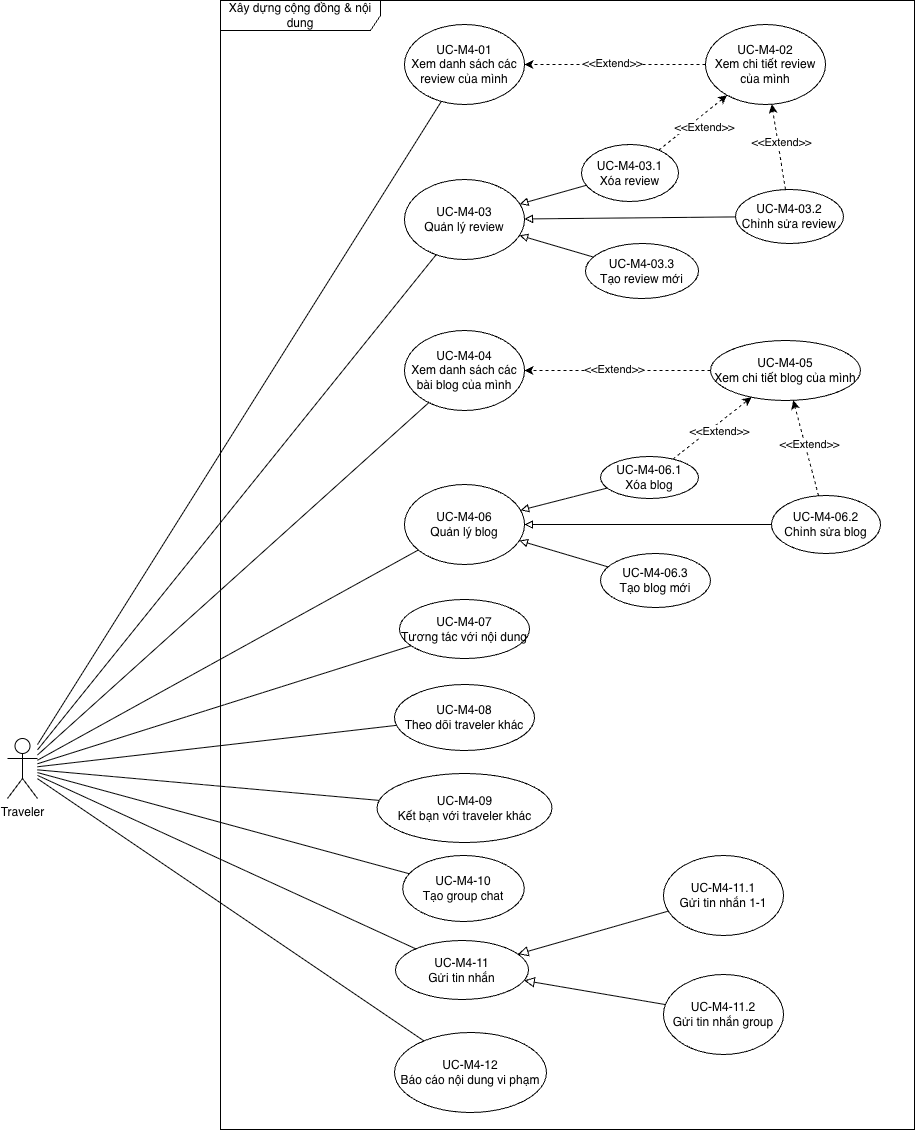
\includegraphics[width=0.9\textwidth]{Images/6. System analysis/4.png}
    \caption{Use case diagram cho Module 4: Xây dựng cộng đồng \& nội dung}
    \label{fig:use_case_module_4}
\end{figure}
% --- //////////////////////////////////////////////////////////////// ---
% MODULE 4
\begin{longtable}{@{}p{4cm} p{11cm}@{}}
\caption{Mô tả Use Case: Xem danh sách các review của mình}
\label{usecase-4-01} \\
\toprule
\textbf{Use case ID}       & UC-M4-01 \\ \midrule
\textbf{Tên Use case}      & Xem danh sách các review của mình \\ \midrule
\textbf{Các tác nhân}      & Traveler \\ \midrule
\textbf{Mô tả}             & Cho phép Traveler xem lại một danh sách tập trung tất cả các bài đánh giá (review) mà họ đã viết cho các địa điểm khác nhau. \\ \midrule
\textbf{Tiền điều kiện}    & Traveler đã đăng nhập vào hệ thống. \\ \midrule
\textbf{Hậu điều kiện}     & Traveler xem được danh sách các review của mình và có thể điều hướng đến từng review hoặc địa điểm tương ứng. \\ \midrule
\textbf{Luồng sự kiện chính} & 
\begin{tabular}[t]{@{}p{10.5cm}@{}}
1. Traveler truy cập vào trang cá nhân và chọn mục ""Các review của tôi"".\\
2. Hệ thống truy vấn cơ sở dữ liệu để lấy tất cả các review do Traveler này tạo.\\
3. Hệ thống hiển thị một danh sách các review, mỗi mục trong danh sách bao gồm: tên địa điểm đã review, điểm đánh giá (số sao), một phần nội dung review và ngày đăng.\\
4. Traveler có thể nhấn vào một review để xem chi tiết trang địa điểm tương ứng, nơi họ có thể thực hiện các hành động trong UC-M3-02 Quản lý Review (chỉnh sửa, xóa).
\end{tabular} \\ \midrule
\textbf{Luồng rẽ nhánh} &
\begin{tabular}[t]{@{}p{10.5cm}@{}}
\textbf{A1: Lọc hoặc sắp xếp danh sách:}\\
1a. Traveler sử dụng công cụ lọc/sắp xếp có sẵn.\\
2a. Traveler có thể sắp xếp danh sách theo tiêu chí như: mới nhất, cũ nhất, điểm đánh giá cao đến thấp (hoặc ngược lại).\\
3a. Hệ thống tải lại danh sách theo tiêu chí đã chọn.
\end{tabular} \\ \midrule
\textbf{Luồng ngoại lệ} &
\begin{tabular}[t]{@{}p{10.5cm}@{}}
\textbf{E1: Người dùng chưa có review nào:}\\
Luồng này xảy ra tại bước 2:\\
2a. Hệ thống không tìm thấy review nào được tạo bởi Traveler.\\
2b. Hệ thống hiển thị thông báo ""Bạn chưa có bài đánh giá nào"".
\end{tabular} \\ 
\bottomrule
\end{longtable}

\begin{longtable}{@{}p{4cm} p{11cm}@{}}
\caption{Mô tả Use Case: Quản lý Review}
\label{usecase-4-03} \\
\toprule
\textbf{Use case ID}       & UC-M4-03 \\ \midrule
\textbf{Tên Use case}      & Quản lý Review \\ \midrule
\textbf{Các tác nhân}      & Traveler \\ \midrule
\textbf{Mô tả}             & Cho phép Traveler tạo một bài đánh giá (review) mới cho một địa điểm (POI), đính kèm media (tối đa 10 ảnh hoặc 1 video), cũng như chỉnh sửa hoặc xóa review của chính mình. \\ \midrule
\textbf{Tiền điều kiện}    & 
\begin{tabular}[t]{@{}p{10.5cm}@{}}
1. Traveler đã đăng nhập vào hệ thống.\\
2. Traveler đang ở trang chi tiết của một địa điểm (Point of Interest - POI) mà họ muốn review.
\end{tabular} \\ \midrule
\textbf{Hậu điều kiện}     & Một review mới được tạo / một review cũ được cập nhật hoặc xóa khỏi hệ thống. Điểm đánh giá trung bình của POI có thể được tính toán lại. \\ \midrule
\textbf{Luồng sự kiện chính} & 
\begin{tabular}[t]{@{}p{10.5cm}@{}}
1. Trên trang chi tiết POI, Traveler nhấn vào nút ""Viết Review"".\\
2. Hệ thống hiển thị một biểu mẫu (form) bao gồm các trường:\\
– Chọn điểm đánh giá (Rating: 1-5 sao).\\
– Ô nhập văn bản cho nội dung review.\\
– Công cụ tải lên media (ảnh/video).\\
3. Traveler chọn số sao, nhập nội dung và tùy chọn tải lên tối đa 10 ảnh hoặc 1 video.\\
4. Traveler nhấn nút ""Đăng"" (Submit).\\
5. Hệ thống kiểm tra tính hợp lệ của dữ liệu (ví dụ: bắt buộc phải có rating, nội dung không được để trống, media đúng định dạng và số lượng).\\
6. Hệ thống lưu review mới vào cơ sở dữ liệu, liên kết nó với tài khoản của Traveler và POI tương ứng.\\
7. Hệ thống hiển thị review mới của Traveler trong danh sách review của POI và thông báo đăng thành công.
\end{tabular} \\ \midrule
\textbf{Luồng rẽ nhánh} &
\begin{tabular}[t]{@{}p{10.5cm}@{}}
\textbf{A1: Chỉnh sửa một review đã có:}\\
1a. Traveler tìm thấy review của chính mình trong danh sách và nhấn vào nút/biểu tượng ""Chỉnh sửa"".\\
2a. Hệ thống hiển thị lại biểu mẫu ở bước 2 của luồng chính, nhưng đã điền sẵn nội dung cũ.\\
3a. Traveler thay đổi nội dung (rating, văn bản, media).\\
4a. Luồng hợp nhất và tiếp tục từ bước 4 của Luồng sự kiện chính.\\
\textbf{A2: Xóa một review đã có:}\\
1b. Traveler tìm thấy review của chính mình và nhấn vào nút/biểu tượng ""Xóa"".\\
2b. Hệ thống hiển thị một hộp thoại yêu cầu xác nhận (ví dụ: ""Bạn có chắc chắn muốn xóa review này không?"").\\
3b. Traveler xác nhận đồng ý.\\
4b. Hệ thống xóa vĩnh viễn review khỏi cơ sở dữ liệu.\\
5b. Hệ thống tải lại danh sách review và hiển thị thông báo ""Đã xóa review thành công"". Use case kết thúc.
\end{tabular} \\ \midrule
\textbf{Luồng ngoại lệ} &
\begin{tabular}[t]{@{}p{10.5cm}@{}}
\textbf{E1: Dữ liệu nhập không hợp lệ}\\
Luồng này xảy ra tại bước 5 của Luồng sự kiện chính:\\
5a. Hệ thống phát hiện lỗi (ví dụ: Traveler chưa chọn rating).\\
5b. Hệ thống chặn việc đăng và hiển thị thông báo lỗi ngay cạnh trường nhập liệu không hợp lệ. Use case tạm dừng cho đến khi Traveler sửa lỗi.\\[3pt]
\textbf{E2: Tải lên media thất bại}\\
Luồng này xảy ra tại bước 3:\\
3a. Quá trình tải media thất bại (do file quá lớn, sai định dạng, mất kết nối).\\
3b. Hệ thống hiển thị thông báo lỗi về việc tải media, cho phép Traveler thử lại hoặc tiếp tục đăng review mà không có media đó.\\[3pt]
\textbf{E3: Lỗi hệ thống khi đăng review}\\
Luồng này xảy ra tại bước 6:\\
6a. Hệ thống không thể lưu review vào cơ sở dữ liệu.\\
6b. Hệ thống hiển thị thông báo lỗi chung (ví dụ: ""Đăng review thất bại, vui lòng thử lại.""). Dữ liệu Traveler đã nhập không bị mất để họ có thể thử lại. Use case kết thúc.
\end{tabular} \\ 
\bottomrule
\end{longtable}

\begin{longtable}{@{}p{4cm} p{11cm}@{}}
\caption{Mô tả Use Case: Xem danh sách các bài blog của mình}
\label{usecase-4-04} \\
\toprule
\textbf{Use case ID}       & UC-M4-04 \\ \midrule
\textbf{Tên Use case}      & Xem danh sách các bài blog của mình \\ \midrule
\textbf{Các tác nhân}      & Traveler \\ \midrule
\textbf{Mô tả}             & Cho phép Traveler xem và quản lý tất cả các bài viết blog mà họ đã tạo, bao gồm cả các bài đã xuất bản và các bản nháp chưa hoàn thành. \\ \midrule
\textbf{Tiền điều kiện}    & Traveler đã đăng nhập vào hệ thống. \\ \midrule
\textbf{Hậu điều kiện}     & Traveler xem được danh sách các bài blog của mình và có thể thực hiện các thao tác quản lý. \\ \midrule
\textbf{Luồng sự kiện chính} & 
\begin{tabular}[t]{@{}p{10.5cm}@{}}
1. Traveler truy cập vào trang cá nhân và chọn mục ""Các bài viết của tôi"".\\
2. Hệ thống truy vấn cơ sở dữ liệu để lấy tất cả các bài viết do Traveler này tạo.\\
3. Hệ thống hiển thị danh sách các bài viết, mỗi mục trong danh sách ghi rõ tiêu đề, ngày cập nhật cuối cùng và trạng thái (""Đã xuất bản"" hoặc ""Bản nháp"").\\
4. Traveler có thể nhấn vào một bài viết để xem chi tiết hoặc thực hiện các hành động trong UC-M3-04 Quản lý Blog (chỉnh sửa, xóa).
\end{tabular} \\ \midrule
\textbf{Luồng rẽ nhánh} &
\begin{tabular}[t]{@{}p{10.5cm}@{}}
\textbf{A1: Lọc danh sách theo trạng thái:}\\
1a. Traveler sử dụng bộ lọc để chọn xem.\\
2a. Hệ thống tải lại danh sách bài viết theo trạng thái đã chọn.
\end{tabular} \\ \midrule
\textbf{Luồng ngoại lệ} &
\begin{tabular}[t]{@{}p{10.5cm}@{}}
\textbf{E1: Người dùng chưa có bài viết nào:}\\
Luồng này xảy ra tại bước 2:\\
2a. Hệ thống không tìm thấy bài viết nào được tạo bởi Traveler.\\
2b. Hệ thống hiển thị thông báo ""Bạn chưa có bài viết nào"" và kèm một nút ""Viết bài mới"".
\end{tabular} \\ 
\bottomrule
\end{longtable}

\begin{longtable}{@{}p{4cm} p{11cm}@{}}
\caption{Mô tả Use Case: Quản lý Blog}
\label{usecase-4-06} \\
\toprule
\textbf{Use case ID}       & UC-M4-06 \\ \midrule
\textbf{Tên Use case}      & Quản lý Blog \\ \midrule
\textbf{Các tác nhân}      & Traveler \\ \midrule
\textbf{Mô tả}             & Cho phép Traveler tạo một bài viết chia sẻ hành trình (dạng blog), lưu lại dưới dạng bản nháp để chỉnh sửa sau, xuất bản bài viết, cũng như cập nhật hoặc xóa bài viết của chính mình. \\ \midrule
\textbf{Tiền điều kiện}    & 
\begin{tabular}[t]{@{}p{10.5cm}@{}}
1. Traveler đã đăng nhập vào hệ thống.\\
2. Traveler đang ở trang tạo bài viết mới hoặc trang quản lý các bài viết của mình.
\end{tabular} \\ \midrule
\textbf{Hậu điều kiện}     & Một bài viết mới được tạo (dưới dạng nháp hoặc đã xuất bản) / một bài viết cũ được cập nhật hoặc xóa khỏi hệ thống. \\ \midrule
\textbf{Luồng sự kiện chính} & 
\begin{tabular}[t]{@{}p{10.5cm}@{}}
1. Traveler truy cập vào chức năng ""Viết bài mới"".\\
2. Hệ thống hiển thị một trình soạn thảo văn bản (rich-text editor) với các trường: ""Tiêu đề"", ""Nội dung"", và các công cụ định dạng, chèn media.\\
3. Traveler nhập tiêu đề, soạn nội dung và chèn media (hình ảnh/video) vào bài viết.\\
4. Traveler nhấn nút ""Xuất bản"" (Publish).\\
5. Hệ thống kiểm tra tính hợp lệ của dữ liệu (ví dụ: tiêu đề và nội dung không được để trống).\\
6. Hệ thống lưu bài viết vào cơ sở dữ liệu với trạng thái ""Đã xuất bản"".\\
7. Hệ thống chuyển hướng Traveler đến trang xem bài viết vừa đăng và hiển thị thông báo ""Xuất bản thành công!""
\end{tabular} \\ \midrule
\textbf{Luồng rẽ nhánh} &
\begin{tabular}[t]{@{}p{10.5cm}@{}}
\textbf{A1: Lưu bài viết dưới dạng Nháp}\\
Luồng này xảy ra tại bước 4 của Luồng sự kiện chính:\\
4a. Thay vì ""Xuất bản"", Traveler nhấn nút ""Lưu nháp"" (Save Draft).\\
5a. Hệ thống thực hiện kiểm tra dữ liệu tối thiểu để lưu nháp (ví dụ: chỉ cần có tiêu đề).\\
6a. Hệ thống lưu bài viết vào cơ sở dữ liệu với trạng thái ""Bản nháp"".\\
7a. Hệ thống thông báo ""Đã lưu nháp thành công!"" và có thể chuyển hướng Traveler về trang quản lý bài viết. Use case kết thúc.\\
\textbf{A2: Chỉnh sửa một bài viết đã có (Nháp hoặc đã xuất bản)}\\
1b. Traveler tìm đến bài viết của mình trong trang quản lý và nhấn ""Chỉnh sửa"".\\
2b. Hệ thống hiển thị lại trình soạn thảo đã điền sẵn nội dung cũ.\\
3b. Traveler thay đổi nội dung.\\
4b. Luồng hợp nhất và tiếp tục từ bước 4 của Luồng sự kiện chính, Traveler có thể chọn ""Lưu nháp"" hoặc ""Xuất bản""/""Cập nhật"".\\
\textbf{A3: Xóa một bài viết:}\\
1c. Traveler tìm đến bài viết của mình và nhấn ""Xóa"".\\
2c. Hệ thống hiển thị hộp thoại yêu cầu xác nhận.\\
3c. Traveler xác nhận đồng ý.\\
4c. Hệ thống xóa bài viết khỏi cơ sở dữ liệu.\\
5c. Hệ thống tải lại danh sách bài viết và hiển thị thông báo ""Đã xóa bài viết thành công"". Use case kết thúc.
\end{tabular} \\ \midrule
\textbf{Luồng ngoại lệ} &
\begin{tabular}[t]{@{}p{10.5cm}@{}}
\textbf{E1: Dữ liệu không hợp lệ khi Xuất bản:}\\
Luồng này xảy ra tại bước 5 của Luồng sự kiện chính:\\
5a. Hệ thống phát hiện lỗi (ví dụ: Traveler chưa nhập tiêu đề).\\
5b. Hệ thống chặn việc xuất bản và hiển thị thông báo lỗi ngay cạnh trường nhập liệu không hợp lệ.\\[3pt]
\textbf{E2: Tải lên media thất bại:}\\
Luồng này xảy ra tại bước 3:\\
3a. Quá trình tải media thất bại (do file quá lớn, sai định dạng, mất kết nối).\\
3b. Hệ thống hiển thị thông báo lỗi, cho phép Traveler thử lại hoặc tiếp tục soạn thảo.\\[3pt]
\textbf{E3: Lỗi hệ thống khi lưu/xuất bản:}\\
Luồng này xảy ra tại bước 6:\\
6a. Hệ thống không thể lưu bài viết vào cơ sở dữ liệu.\\
6b. Hệ thống hiển thị thông báo lỗi chung và giữ lại nội dung Traveler đã soạn để tránh mất dữ liệu. Use case kết thúc.
\end{tabular} \\ 
\bottomrule
\end{longtable}

\begin{longtable}{@{}p{4cm} p{11cm}@{}}
\caption{Mô tả Use Case: Tương tác với nội dung}
\label{usecase-4-07} \\
\toprule
\textbf{Use case ID}       & UC-M4-07 \\ \midrule
\textbf{Tên Use case}      & Tương tác với nội dung \\ \midrule
\textbf{Các tác nhân}      & Traveler \\ \midrule
\textbf{Mô tả}             & Cho phép Traveler tương tác với một bài viết hoặc review thông qua các hành động: để lại bình luận, bày tỏ cảm xúc (react), hoặc lưu lại bài viết đó để xem sau. \\ \midrule
\textbf{Tiền điều kiện}    & 
\begin{tabular}[t]{@{}p{10.5cm}@{}}
1. Traveler đã đăng nhập vào hệ thống.\\
2. Traveler đang ở trang xem chi tiết một bài viết.
\end{tabular} \\ \midrule
\textbf{Hậu điều kiện}     & Tương tác của Traveler (bình luận, cảm xúc, lưu) được ghi nhận vào hệ thống và giao diện được cập nhật để phản ánh sự thay đổi đó. \\ \midrule
\textbf{Luồng sự kiện chính} & 
\begin{tabular}[t]{@{}p{10.5cm}@{}}
1. Traveler kéo xuống phần bình luận của bài viết/review.\\
2. Traveler nhập nội dung bình luận vào ô soạn thảo.\\
3. Traveler nhấn nút ""Gửi"" (Post).\\
4. Hệ thống kiểm tra tính hợp lệ của bình luận (ví dụ: không được để trống, không chứa từ khóa bị cấm).\\
5. Hệ thống lưu bình luận vào cơ sở dữ liệu, liên kết nó với Traveler và nội dung đang xem.\\
6. Hệ thống cập nhật lại danh sách bình luận ngay lập tức để hiển thị bình luận mới của Traveler.
\end{tabular} \\ \midrule
\textbf{Luồng rẽ nhánh} &
\begin{tabular}[t]{@{}p{10.5cm}@{}}
\textbf{A1: Bày tỏ cảm xúc (React) với nội dung:}\\
1a. Traveler nhấn vào nút/biểu tượng cảm xúc (ví dụ: Thích, Tim, Haha).\\
2a. Hệ thống ngay lập tức ghi nhận cảm xúc đó vào cơ sở dữ liệu.\\
3a. Giao diện cập nhật lại trạng thái của nút bấm (ví dụ: chuyển sang màu xanh) và tăng tổng số lượt cảm xúc.\\
4. (Sub-flow) Bỏ bày tỏ cảm xúc: Nếu Traveler nhấn lại vào nút đó, hệ thống sẽ xóa lượt cảm xúc và giao diện trở về trạng thái ban đầu.\\
\textbf{A2: Lưu (Bookmark) nội dung để xem sau:}\\
1b. Traveler nhấn vào nút/biểu tượng ""Lưu"" (Save/Bookmark).\\
2b. Hệ thống thêm bài viết/review này vào danh sách ""Đã lưu"" của Traveler.\\
3b. Giao diện cập nhật lại trạng thái của nút bấm (ví dụ: biểu tượng được tô đầy).\\
4b. (Sub-flow) Bỏ lưu: Nếu Traveler nhấn lại vào nút đó, hệ thống sẽ xóa nội dung khỏi danh sách ""Đã lưu"" và giao diện trở về trạng thái ban đầu.\\
\textbf{A3: Chỉnh sửa hoặc Xóa bình luận của chính mình}\\
1c. Traveler tìm đến một bình luận do chính mình đã đăng.\\
2c. Traveler nhấn vào tùy chọn ""Chỉnh sửa"" hoặc ""Xóa"".\\
3c. Nếu ""Chỉnh sửa"", hệ thống cho phép sửa lại nội dung và lưu lại. Nếu ""Xóa"", hệ thống yêu cầu xác nhận và sau đó xóa bình luận.
\end{tabular} \\ \midrule
\textbf{Luồng ngoại lệ} &
\begin{tabular}[t]{@{}p{10.5cm}@{}}
\textbf{E1: Nội dung bình luận không hợp lệ:}\\
Luồng này xảy ra tại bước 4 của Luồng sự kiện chính:\\
4a. Hệ thống phát hiện bình luận vi phạm (trống, chứa spam,...).\\
4b. Hệ thống chặn việc gửi và hiển thị thông báo lỗi (ví dụ: ""Bình luận không được để trống"").\\[3pt]
\textbf{E2: Lỗi kết nối hoặc lỗi máy chủ:}\\
Luồng này có thể xảy ra khi thực hiện bất kỳ tương tác nào (bình luận, thả cảm xúc, lưu):\\
1a. Hệ thống không thể gửi dữ liệu tương tác lên máy chủ.\\
2a. Hệ thống hiển thị thông báo lỗi (ví dụ: ""Tương tác thất bại, vui lòng thử lại"") và không thay đổi trạng thái giao diện.
\end{tabular} \\ 
\bottomrule
\end{longtable}

\begin{longtable}{@{}p{4cm} p{11cm}@{}}
\caption{Mô tả Use Case: Tạo Group Chat}
\label{usecase-4-10} \\
\toprule
\textbf{Use case ID}       & UC-M4-10 \\ \midrule
\textbf{Tên Use case}      & Tạo Group Chat \\ \midrule
\textbf{Các tác nhân}      & Traveler \\ \midrule
\textbf{Mô tả}             & Cho phép Traveler (Người tạo) tạo một nhóm chat mới bằng cách chọn các thành viên từ danh sách bạn bè của mình. \\ \midrule
\textbf{Tiền điều kiện}    & 
\begin{tabular}[t]{@{}p{10.5cm}@{}}
1. Traveler (Người tạo) đã đăng nhập.\\
2. Traveler (Người tạo) có ít nhất một người bạn.
\end{tabular} \\ \midrule
\textbf{Hậu điều kiện}     & 
\begin{tabular}[t]{@{}p{10.5cm}@{}}
(Thành công): Group chat được tạo, các thành viên hợp lệ được thêm vào nhóm.\\
(Thất bại): Group chat không được tạo.
\end{tabular} \\ \midrule
\textbf{Luồng sự kiện chính} & 
\begin{tabular}[t]{@{}p{10.5cm}@{}}
1. Traveler A chọn chức năng ""Tạo Group Chat"".\\
2. Hệ thống hiển thị danh sách bạn bè của Traveler A.\\
3. Traveler A chọn một hoặc nhiều bạn bè từ danh sách này để thêm vào nhóm.\\
4. Traveler A đặt tên cho nhóm (ví dụ: ""Nhóm Du lịch Phú Quốc"").\\
5. Traveler A nhấn ""Tạo nhóm"".\\
6. Hệ thống tạo Group Chat mới với các thành viên đã chọn.\\
7. Hệ thống hiển thị thông báo ""Tạo nhóm thành công"" và mở giao diện chat nhóm.
\end{tabular} \\ \midrule
\textbf{Luồng rẽ nhánh}    & (Không có) \\ \midrule
\textbf{Luồng ngoại lệ} &
\begin{tabular}[t]{@{}p{10.5cm}@{}}
\textbf{E1: Không chọn thành viên:}\\
Tại bước 5, Traveler nhấn ""Tạo nhóm"" nhưng chưa chọn bất kỳ người bạn nào.\\
Hệ thống hiển thị thông báo ""Vui lòng chọn ít nhất hai thành viên cho nhóm.""\\[3pt]
\textbf{E2: Lỗi hệ thống:}\\
Tại bước 6, hệ thống không thể tạo nhóm do lỗi CSDL.\\
Hệ thống hiển thị thông báo ""Đã xảy ra lỗi, không thể tạo nhóm. Vui lòng thử lại sau.""
\end{tabular} \\ 
\bottomrule
\end{longtable}

\begin{longtable}{@{}p{4cm} p{11cm}@{}}
\caption{Mô tả Use Case: Gửi tin nhắn 1-1}
\label{usecase-4-11-1} \\
\toprule
\textbf{Use case ID}       & UC-M4-11.1 \\ \midrule
\textbf{Tên Use case}      & Gửi tin nhắn 1-1 \\ \midrule
\textbf{Các tác nhân}      & Traveler \\ \midrule
\textbf{Mô tả}             & Cho phép một Traveler (người gửi) gửi một tin nhắn riêng tư cho một Traveler khác (người nhận) trong hệ thống. Use case này bao gồm việc xem lại lịch sử trò chuyện và gửi tin nhắn mới. \\ \midrule
\textbf{Tiền điều kiện}    & 
\begin{tabular}[t]{@{}p{10.5cm}@{}}
1. Traveler (người gửi) đã đăng nhập vào hệ thống.\\
2. Traveler đã truy cập vào mục ""Tin nhắn"" hoặc trang cá nhân của người muốn gửi tin.
\end{tabular} \\ \midrule
\textbf{Hậu điều kiện}     & Tin nhắn được gửi thành công, hiển thị trong cuộc trò chuyện của cả người gửi và người nhận. \\ \midrule
\textbf{Luồng sự kiện chính} & 
\begin{tabular}[t]{@{}p{10.5cm}@{}}
1. Traveler (Người gửi) mở cuộc trò chuyện với một Traveler khác (Người nhận).\\
2. Hệ thống tải và hiển thị lịch sử tin nhắn trước đó giữa hai người (nếu có).\\
3. Người gửi nhập nội dung tin nhắn vào ô soạn thảo.\\
4. Người gửi nhấn nút ""Gửi"".\\
5. Hệ thống kiểm tra tính hợp lệ của tin nhắn (ví dụ: không được để trống, không vi phạm bộ lọc từ khóa).\\
6. Hệ thống lưu tin nhắn vào cơ sở dữ liệu.\\
7. Hệ thống cập nhật giao diện trò chuyện của Người gửi ngay lập tức để hiển thị tin nhắn vừa gửi.\\
8. Hệ thống gửi tin nhắn (và có thể kèm một thông báo ""có tin nhắn mới"") đến cho Người nhận.
\end{tabular} \\ \midrule
\textbf{Luồng rẽ nhánh} &
\begin{tabular}[t]{@{}p{10.5cm}@{}}
\textbf{A1: Bắt đầu một cuộc trò chuyện mới:}\\
Luồng này xảy ra khi chưa có lịch sử trò chuyện giữa hai người:\\
1a. Traveler (Người gửi) vào trang cá nhân của Traveler khác và nhấn nút ""Nhắn tin"".\\
2a. Hệ thống mở một cửa sổ trò chuyện trống.\\
3a. Luồng hợp nhất và tiếp tục từ bước 3 của Luồng sự kiện chính.
\end{tabular} \\ \midrule
\textbf{Luồng ngoại lệ} &
\begin{tabular}[t]{@{}p{10.5cm}@{}}
\textbf{E1: Lỗi kết nối hoặc lỗi máy chủ:}\\
Luồng này xảy ra tại bước 6:\\
6a. Hệ thống không thể gửi tin nhắn lên máy chủ.\\
6b. Hệ thống hiển thị trạng thái ""Gửi thất bại"" bên cạnh tin nhắn đó và có thể cung cấp tùy chọn ""Thử lại"".\\[3pt]
\textbf{E2: Người nhận đã chặn người gửi:}\\
Luồng này xảy ra tại bước 4:\\
4a. Hệ thống kiểm tra và phát hiện Người nhận đã chặn Người gửi.\\
4b. Hệ thống chặn việc gửi và hiển thị thông báo ""Bạn không thể gửi tin nhắn cho người dùng này"". Use case kết thúc.
\end{tabular} \\ 
\bottomrule
\end{longtable}

\begin{longtable}{@{}p{4cm} p{11cm}@{}}
\caption{Mô tả Use Case: Gửi tin nhắn Group}
\label{usecase-4-11-2} \\
\toprule
\textbf{Use case ID}       & UC-M4-11.2 \\ \midrule
\textbf{Tên Use case}      & Gửi tin nhắn Group \\ \midrule
\textbf{Các tác nhân}      & Traveler \\ \midrule
\textbf{Mô tả}             & Cho phép Traveler gửi tin nhắn vào một Group Chat mà họ là thành viên \\ \midrule
\textbf{Tiền điều kiện}    & 
\begin{tabular}[t]{@{}p{10.5cm}@{}}
1. Traveler đã đăng nhập.\\
2. Traveler là thành viên của Group Chat.
\end{tabular} \\ \midrule
\textbf{Hậu điều kiện}     & 
\begin{tabular}[t]{@{}p{10.5cm}@{}}
1. Tin nhắn được gửi thành công và lưu vào CSDL.\\
2. Tất cả thành viên khác trong nhóm nhận được tin nhắn.
\end{tabular} \\ \midrule
\textbf{Luồng sự kiện chính} & 
\begin{tabular}[t]{@{}p{10.5cm}@{}}
1. Traveler A mở danh sách nhóm chat và chọn ""Nhóm Du lịch Phú Quốc"".\\
2. Hệ thống kiểm tra Tiền điều kiện 2 (xác nhận Traveler A vẫn là thành viên).\\
3. Hệ thống mở giao diện chat nhóm.\\
4. Traveler A nhập nội dung tin nhắn và nhấn ""Gửi"".\\
5. Hệ thống lưu tin nhắn vào CSDL, liên kết với ID của nhóm.\\
6. Hệ thống đẩy tin nhắn (broadcast) đến tất cả thành viên khác của nhóm.
\end{tabular} \\ \midrule
\textbf{Luồng rẽ nhánh}    & (Không có) \\ \midrule
\textbf{Luồng ngoại lệ} &
\begin{tabular}[t]{@{}p{10.5cm}@{}}
\textbf{E1: Bị xóa khỏi nhóm:}\\
Tại bước 2, hệ thống phát hiện Traveler A không (hoặc không còn) là thành viên của nhóm.\\
Hệ thống hiển thị thông báo ""Bạn không còn là thành viên của nhóm này."" Use case kết thúc.
\end{tabular} \\ 
\bottomrule
\end{longtable}

\begin{longtable}{@{}p{4cm} p{11cm}@{}}
\caption{Mô tả Use Case: Báo cáo nội dung vi phạm}
\label{usecase-4-12} \\
\toprule
\textbf{Use case ID}       & UC-M4-12 \\ \midrule
\textbf{Tên Use case}      & Báo cáo nội dung vi phạm \\ \midrule
\textbf{Các tác nhân}      & Traveler \\ \midrule
\textbf{Mô tả}             & Cho phép Traveler gửi một báo cáo (report) về một nội dung (bài viết, review, bình luận) mà họ cho là vi phạm tiêu chuẩn cộng đồng. Báo cáo này sẽ được gửi đến đội ngũ quản trị viên (Moderator/Admin) để xem xét. \\ \midrule
\textbf{Tiền điều kiện}    & 
\begin{tabular}[t]{@{}p{10.5cm}@{}}
1. Traveler đã đăng nhập vào hệ thống.\\
2. Traveler đang xem một nội dung cụ thể (bài viết, review, bình luận).
\end{tabular} \\ \midrule
\textbf{Hậu điều kiện}     & Một báo cáo mới được tạo trong hàng đợi xử lý của quản trị viên, và Traveler nhận được thông báo xác nhận. \\ \midrule
\textbf{Luồng sự kiện chính} & 
\begin{tabular}[t]{@{}p{10.5cm}@{}}
1. Traveler tìm thấy một nội dung mà họ cho là vi phạm.\\
2. Traveler nhấn vào tùy chọn ""Báo cáo"" (thường nằm trong menu ""..."").\\
3. Hệ thống hiển thị một biểu mẫu (form) với danh sách các lý do báo cáo (ví dụ: ""Spam"", ""Nội dung không phù hợp"", ""Thông tin sai sự thật"", ""Quấy rối"",...).\\
4. Traveler chọn một hoặc nhiều lý do phù hợp. Hệ thống có thể cung cấp thêm một ô văn bản để Traveler mô tả chi tiết hơn.\\
5. Traveler nhấn nút ""Gửi báo cáo"".\\
6. Hệ thống kiểm tra tính hợp lệ (bắt buộc phải chọn ít nhất một lý do).\\
7. Hệ thống tạo một bản ghi báo cáo mới trong cơ sở dữ liệu, bao gồm thông tin về người báo cáo, nội dung bị báo cáo, và lý do.\\
8. Hệ thống hiển thị một thông báo xác nhận cho Traveler (ví dụ: ""Cảm ơn bạn đã báo cáo. Đội ngũ quản trị sẽ xem xét trường hợp này."").
\end{tabular} \\ \midrule
\textbf{Luồng rẽ nhánh}    & Không có \\ \midrule
\textbf{Luồng ngoại lệ} &
\begin{tabular}[t]{@{}p{10.5cm}@{}}
\textbf{E1: Người dùng không chọn lý do báo cáo:}\\
Luồng này xảy ra tại bước 6 của Luồng sự kiện chính:\\
6a. Hệ thống phát hiện Traveler chưa chọn lý do nào.\\
6b. Hệ thống chặn việc gửi và hiển thị thông báo lỗi: ""Vui lòng chọn ít nhất một lý do báo cáo.""\\[3pt]
\textbf{E2: Lỗi kết nối hoặc lỗi máy chủ:}\\
Luồng này xảy ra tại bước 7:\\
7a. Hệ thống không thể lưu báo cáo vào cơ sở dữ liệu.\\
7b. Hệ thống hiển thị thông báo lỗi chung: ""Gửi báo cáo thất bại, vui lòng thử lại sau."" Use case kết thúc.\\[3pt]
\textbf{E3: Nội dung bị xóa trong khi đang báo cáo:}\\
Luồng này xảy ra khi nội dung bị xóa bởi tác giả hoặc quản trị viên trong khoảng thời gian từ bước 2 đến bước 5:\\
7c. Tại bước 7, hệ thống không tìm thấy nội dung được liên kết để tạo báo cáo.\\
7d. Hệ thống hiển thị thông báo lỗi: ""Nội dung này không còn tồn tại."" Use case kết thúc.
\end{tabular} \\ 
\bottomrule
\end{longtable}


% --- 6. MODULE 5: QUẢN LÝ NỘI DUNG ---
\subsubsubsection{Module 5: Quản lý nội dung}
\begin{figure}[H]
    \centering
    % NOTE: Bổ sung tên file ảnh cho Module 5 (Quản lý nội dung)
    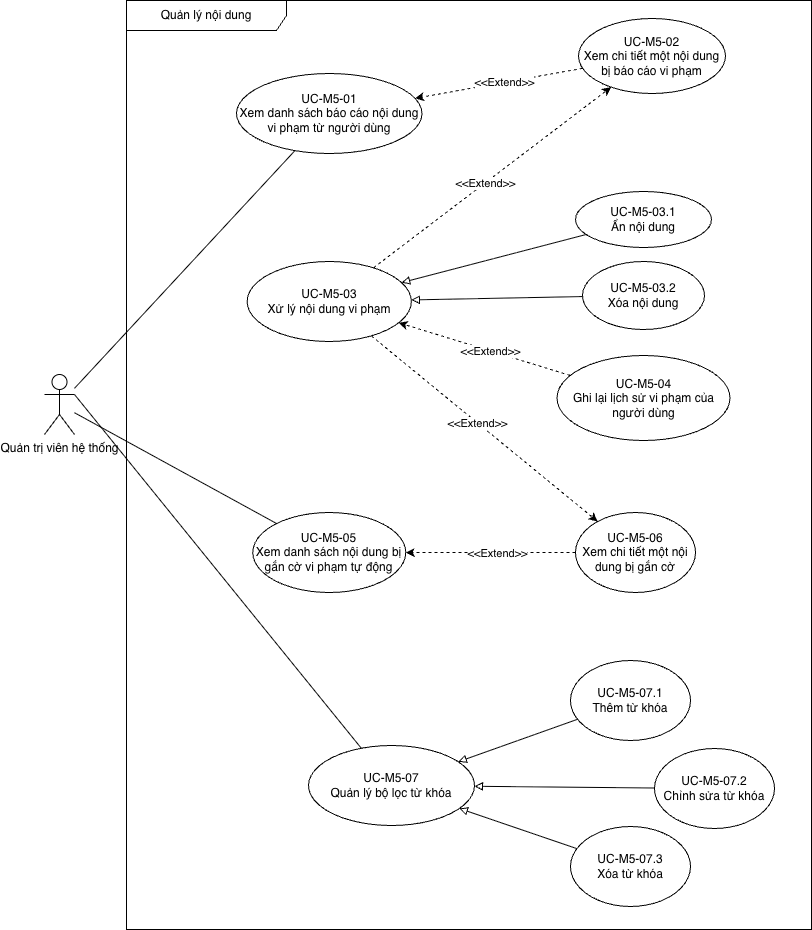
\includegraphics[width=0.9\textwidth]{Images/6. System analysis/5.png}
    \caption{Use case diagram cho Module 5: Quản lý nội dung}
    \label{fig:use_case_module_5}
\end{figure}
% --- //////////////////////////////////////////////////////////////// ---
% MODULE 5
\begin{longtable}{@{}p{4cm} p{11cm}@{}}
\caption{Mô tả Use Case: Xem danh sách báo cáo nội dung vi phạm từ người dùng}
\label{usecase-5-01} \\
\toprule
\textbf{Use case ID}       & UC-M5-01 \\ \midrule
\textbf{Tên Use case}      & Xem danh sách báo cáo nội dung vi phạm từ người dùng \\ \midrule
\textbf{Các tác nhân}      & Quản trị viên cộng đồng \\ \midrule
\textbf{Mô tả}             & Cho phép Admin xem lại các báo cáo vi phạm do người dùng ( Traveler ) gửi lên, đánh giá nội dung bị báo cáo và đưa ra các hành động xử lý phù hợp. \\ \midrule
\textbf{Tiền điều kiện}    & 
\begin{tabular}[t]{@{}p{10.5cm}@{}}
1. Admin đã đăng nhập vào hệ thống với đúng quyền hạn.\\
2. Có ít nhất một báo cáo từ người dùng đang ở trạng thái ""chờ xử lý"" trong hệ thống.
\end{tabular} \\ \midrule
\textbf{Hậu điều kiện}     & Báo cáo được cập nhật trạng thái (ví dụ: ""Đã xử lý"", ""Bỏ qua""). Nội dung vi phạm có thể bị ẩn/xóa. \\ \midrule
\textbf{Luồng sự kiện chính} & 
\begin{tabular}[t]{@{}p{10.5cm}@{}}
1. Admin truy cập vào trang ""Quản lý Báo cáo"" (Moderation Queue).\\
2. Hệ thống hiển thị một danh sách các báo cáo đang chờ xử lý, sắp xếp theo thứ tự ưu tiên (ví dụ: mới nhất, hoặc nhiều lượt báo cáo nhất).\\
3. Admin chọn một báo cáo cụ thể để xem chi tiết.\\
4. Hệ thống hiển thị đầy đủ thông tin của báo cáo, bao gồm:\\
– Nội dung bị báo cáo (bình luận, review, bài viết).\\
– Lý do người dùng báo cáo.\\
– Ghi chú chi tiết từ người báo cáo (nếu có).\\
– Liên kết để xem nội dung trong ngữ cảnh gốc.\\
5. Admin xem xét nội dung và xác định mức độ vi phạm.\\
6. Admin chọn một hành động để xử lý nội dung, ví dụ: ""Ẩn nội dung"" hoặc ""Xóa nội dung"" .\\
7. Hệ thống yêu cầu xác nhận hành động. Admin xác nhận.\\
8. Hệ thống thực thi hành động (ẩn/xóa nội dung khỏi chế độ xem công khai).\\
9. Hệ thống tự động cập nhật trạng thái của báo cáo thành ""Đã xử lý - Vi phạm"".
\end{tabular} \\ \midrule
\textbf{Luồng rẽ nhánh} &
\begin{tabular}[t]{@{}p{10.5cm}@{}}
\textbf{A1: Bỏ qua báo cáo (Không vi phạm):}\\
Luồng này xảy ra tại bước 6 của Luồng sự kiện chính:\\
6a. Admin xác định rằng nội dung không vi phạm chính sách.\\
7a. Họ chọn hành động ""Bỏ qua"" (Dismiss) hoặc ""Không vi phạm"" .\\
8a. Hệ thống cập nhật trạng thái của báo cáo thành ""Đã xử lý - Không vi phạm"" và giữ nguyên nội dung. Use case kết thúc.
\end{tabular} \\ \midrule
\textbf{Luồng ngoại lệ} &
\begin{tabular}[t]{@{}p{10.5cm}@{}}
\textbf{E1: Nội dung đã được xử lý hoặc không còn tồn tại}\\
Luồng này xảy ra tại bước 3:\\
3a. Admin chọn một báo cáo, nhưng nội dung liên quan đã bị xóa (bởi tác giả hoặc một admin khác) hoặc báo cáo đã được xử lý.\\
3b. Hệ thống hiển thị thông báo ""Nội dung này không còn tồn tại hoặc báo cáo đã được xử lý"" và có thể tự động cập nhật trạng thái báo cáo. Use case kết thúc.\\[3pt]
\textbf{E2: Lỗi hệ thống khi thực hiện hành động:}\\
Luồng này xảy ra tại bước 8:\\
8a. Hệ thống gặp lỗi và không thể ẩn/xóa nội dung.\\
8b. Hệ thống hiển thị thông báo lỗi (ví dụ: ""Xử lý thất bại, vui lòng thử lại"") và giữ nguyên trạng thái của báo cáo.
\end{tabular} \\ 
\bottomrule
\end{longtable}

\begin{longtable}{@{}p{4cm} p{11cm}@{}}
\caption{Mô tả Use Case: Ghi lại Lịch sử Vi phạm}
\label{usecase-5-04} \\
\toprule
\textbf{Use case ID}       & UC-M5-04 \\ \midrule
\textbf{Tên Use case}      & Ghi lại Lịch sử Vi phạm \\ \midrule
\textbf{Các tác nhân}      & (Không có Primary Actor - Included Use Case) \\ \midrule
\textbf{Mô tả}             & Sub-use case bắt buộc, được <<include>> bởi các Use Case xử lý nội dung vi phạm (như Ẩn nội dung , Xóa nội dung ). Tự động tạo bản ghi vi phạm liên kết với người dùng để Module 8 sử dụng. \\ \midrule
\textbf{Tiền điều kiện}    & 
\begin{tabular}[t]{@{}p{10.5cm}@{}}
1. Use Case cha (ví dụ: Ẩn nội dung ) đã được kích hoạt và xác nhận.\\
2. Hệ thống đã xác định được ID người dùng (tác giả) vi phạm.
\end{tabular} \\ \midrule
\textbf{Hậu điều kiện}     & 
\begin{tabular}[t]{@{}p{10.5cm}@{}}
1. (Thành công): Bản ghi VIOLATION\_RECORDS mới được tạo trong CSDL.\\
2. (Thất bại): Lỗi được ghi nhận, Use Case cha bị dừng/thông báo lỗi.
\end{tabular} \\ \midrule
\textbf{Luồng sự kiện chính} & 
\begin{tabular}[t]{@{}p{10.5cm}@{}}
1. Use Case được gọi bởi Use Case cha.\\
2. Hệ thống thu thập thông tin: user\_id , content\_id , reason , admin\_id .\\
3. Hệ thống tạo bản ghi mới trong bảng VIOLATION\_RECORDS .\\
4. Use Case kết thúc thành công, trả quyền kiểm soát về Use Case cha.
\end{tabular} \\ \midrule
\textbf{Luồng rẽ nhánh}    & (Không có) \\ \midrule
\textbf{Luồng ngoại lệ} &
\begin{tabular}[t]{@{}p{10.5cm}@{}}
\textbf{E1: Không tìm thấy User ID:}\\
1a. Tại bước 2, hệ thống không xác định được user\_id .\\
1b. Use Case thất bại. Use Case cha bị dừng và hiển thị lỗi: ""Không thể xử lý vi phạm, không tìm thấy tác giả.""\\[3pt]
\textbf{E2: Lỗi ghi CSDL:}\\
2a. Tại bước 3, hệ thống gặp lỗi khi tạo bản ghi.\\
2b. Use Case thất bại. Use Case cha bị dừng và hiển thị lỗi: ""Ghi nhận lịch sử vi phạm thất bại. Đã xảy ra lỗi hệ thống.""
\end{tabular} \\ 
\bottomrule
\end{longtable}

\begin{longtable}{@{}p{4cm} p{11cm}@{}}
\caption{Mô tả Use Case: Xem danh sách nội dung bị gắn cờ vi phạm tự động}
\label{usecase-5-05} \\
\toprule
\textbf{Use case ID}       & UC-M5-05 \\ \midrule
\textbf{Tên Use case}      & Xem danh sách nội dung bị gắn cờ vi phạm tự động \\ \midrule
\textbf{Các tác nhân}      & Admin \\ \midrule
\textbf{Mô tả}             & Cho phép Admin xem xét danh sách các nội dung (bài viết, review, bình luận) đã bị hệ thống tự động phát hiện và gắn cờ là có khả năng vi phạm (dựa trên bộ lọc từ khóa, AI,...). \\ \midrule
\textbf{Tiền điều kiện}    & 
\begin{tabular}[t]{@{}p{10.5cm}@{}}
1. Admin đã đăng nhập vào hệ thống với đúng quyền hạn.\\
2. Có ít nhất một nội dung đang bị hệ thống tự động gắn cờ và đưa vào hàng đợi kiểm duyệt.
\end{tabular} \\ \midrule
\textbf{Hậu điều kiện}     & Nội dung bị gắn cờ được xử lý (được duyệt đăng, bị ẩn/xóa) và được đưa ra khỏi hàng đợi kiểm duyệt. \\ \midrule
\textbf{Luồng sự kiện chính} & 
\begin{tabular}[t]{@{}p{10.5cm}@{}}
1. Admin truy cập vào trang ""Hàng đợi kiểm duyệt tự động"".\\
2. Hệ thống hiển thị danh sách các nội dung bị gắn cờ, kèm theo lý do bị gắn cờ (ví dụ: ""Chứa từ khóa bị cấm: [từ khóa]"").\\
3. Admin chọn một nội dung để xem xét chi tiết.\\
4. Hệ thống hiển thị đầy đủ nội dung, trong đó làm nổi bật yếu tố đã gây ra cảnh báo (ví dụ: bôi vàng từ khóa bị cấm).\\
5. Admin đánh giá và nhận thấy nội dung không thực sự vi phạm (trường hợp ""false positive"").\\
6. Admin chọn hành động ""Duyệt"" (Approve) hoặc ""Cho phép hiển thị"" .\\
7. Hệ thống yêu cầu xác nhận. Admin xác nhận.\\
8. Hệ thống gỡ cờ khỏi nội dung và cho phép nó hiển thị công khai (nếu trước đó bị tạm ẩn).\\
9. Hệ thống xóa nội dung khỏi hàng đợi kiểm duyệt và hiển thị thông báo ""Đã duyệt nội dung thành công"".
\end{tabular} \\ \midrule
\textbf{Luồng rẽ nhánh} &
\begin{tabular}[t]{@{}p{10.5cm}@{}}
\textbf{A1: Xác nhận vi phạm và xử lý nội dung:}\\
Luồng này xảy ra tại bước 6 của Luồng sự kiện chính:\\
6a. Admin xác định rằng nội dung thực sự vi phạm chính sách.\\
7a. Họ chọn một hành động xử lý, ví dụ: ""Ẩn nội dung"" hoặc ""Xóa nội dung"" .\\
8a. Hệ thống thực thi hành động (ẩn/xóa nội dung).\\
9a. Hệ thống xóa nội dung khỏi hàng đợi và cập nhật trạng thái là ""Đã xử lý - Vi phạm"". Use case kết thúc.\\[3pt]
\textbf{A2: Chỉnh sửa và duyệt nội dung:}\\
Luồng này xảy ra tại bước 6:\\
6b. Admin thấy nội dung chỉ vi phạm nhẹ và có thể sửa được.\\
7b. Họ chọn hành động ""Chỉnh sửa"", sau đó tự tay xóa hoặc thay đổi phần nội dung vi phạm.\\
8b. Sau khi sửa xong, họ nhấn ""Lưu và Duyệt"".\\
9b. Hệ thống lưu lại nội dung đã chỉnh sửa và cho phép hiển thị công khai. Use case kết thúc.
\end{tabular} \\ \midrule
\textbf{Luồng ngoại lệ} &
\begin{tabular}[t]{@{}p{10.5cm}@{}}
\textbf{E1: Nội dung đã được xử lý hoặc không còn tồn tại:}\\
Luồng này xảy ra tại bước 3:\\
3a. Admin chọn một nội dung, nhưng nó đã được một admin khác xử lý hoặc tác giả đã tự xóa.\\
3b. Hệ thống hiển thị thông báo ""Nội dung này không còn tồn tại hoặc đã được xử lý"" và tự động xóa khỏi hàng đợi. Use case kết thúc.\\[3pt]
\textbf{E2: Lỗi hệ thống khi thực hiện hành động:}\\
Luồng này xảy ra tại bước 8 hoặc 8a, 9b:\\
8a. Hệ thống gặp lỗi và không thể thực hiện hành động (duyệt/ẩn/xóa).\\
8b. Hệ thống hiển thị thông báo lỗi và giữ nguyên nội dung trong hàng đợi để xử lý lại sau.
\end{tabular} \\ 
\bottomrule
\end{longtable}

\begin{longtable}{@{}p{4cm} p{11cm}@{}}
\caption{Mô tả Use Case: Quản lý bộ lọc từ khóa}
\label{usecase-5-07} \\
\toprule
\textbf{Use case ID}       & UC-M5-07 \\ \midrule
\textbf{Tên Use case}      & Quản lý bộ lọc từ khóa \\ \midrule
\textbf{Các tác nhân}      & Quản trị viên hệ thống \\ \midrule
\textbf{Mô tả}             & Cho phép Admin quản lý danh sách các từ khóa bị cấm hoặc nhạy cảm. Hệ thống sẽ sử dụng danh sách này làm cơ sở để tự động gắn cờ nội dung vi phạm (trong UC-M4-02). \\ \midrule
\textbf{Tiền điều kiện}    & Admin đã đăng nhập vào hệ thống với quyền quản trị cao nhất và đã truy cập vào khu vực cài đặt kiểm duyệt. \\ \midrule
\textbf{Hậu điều kiện}     & Danh sách từ khóa trong bộ lọc của hệ thống được cập nhật (thêm, sửa, hoặc xóa thành công). \\ \midrule
\textbf{Luồng sự kiện chính} & 
\begin{tabular}[t]{@{}p{10.5cm}@{}}
1. Admin truy cập vào trang ""Quản lý Bộ lọc Từ khóa"".\\
2. Hệ thống hiển thị danh sách tất cả các từ khóa đang có trong bộ lọc.\\
3. Admin nhấn vào nút ""Thêm từ khóa mới"".\\
4. Hệ thống hiển thị một ô nhập liệu để Admin điền từ khóa mới.\\
5. Admin nhập từ khóa và nhấn ""Lưu"".\\
6. Hệ thống kiểm tra tính hợp lệ của từ khóa (ví dụ: không được để trống, không bị trùng lặp).\\
7. Hệ thống lưu từ khóa mới vào cơ sở dữ liệu.\\
8. Hệ thống tải lại danh sách trên giao diện để hiển thị từ khóa vừa thêm và thông báo ""Thêm từ khóa thành công"".
\end{tabular} \\ \midrule
\textbf{Luồng rẽ nhánh} &
\begin{tabular}[t]{@{}p{10.5cm}@{}}
\textbf{A1: Chỉnh sửa một từ khóa đã có:}\\
1a. Admin tìm đến từ khóa muốn sửa trong danh sách và nhấn vào nút/biểu tượng ""Chỉnh sửa"".\\
2a. Hệ thống cho phép Admin chỉnh sửa trực tiếp trên dòng đó hoặc hiển thị một ô nhập liệu với nội dung cũ.\\
3a. Admin thay đổi nội dung từ khóa và nhấn ""Lưu"".\\
4. Luồng hợp nhất và tiếp tục từ bước 6 của Luồng sự kiện chính.\\[3pt]
\textbf{A2: Xóa một từ khóa đã có:}\\
1b. Admin tìm đến từ khóa muốn xóa trong danh sách và nhấn vào nút/biểu tượng ""Xóa"".\\
2b. Hệ thống hiển thị một hộp thoại yêu cầu xác nhận.\\
3b. Admin xác nhận đồng ý.\\
4b. Hệ thống xóa từ khóa khỏi cơ sở dữ liệu.\\
5b. Hệ thống tải lại danh sách và hiển thị thông báo ""Đã xóa từ khóa thành công"". Use case kết thúc.
\end{tabular} \\ \midrule
\textbf{Luồng ngoại lệ} &
\begin{tabular}[t]{@{}p{10.5cm}@{}}
\textbf{E1: Dữ liệu nhập không hợp lệ:}\\
Luồng này xảy ra tại bước 6 của Luồng sự kiện chính:\\
6a. Hệ thống phát hiện Admin nhập một từ khóa đã tồn tại hoặc để trống.\\
6b. Hệ thống chặn việc lưu và hiển thị thông báo lỗi tương ứng (ví dụ: ""Từ khóa này đã tồn tại"" hoặc ""Từ khóa không được để trống"").\\[3pt]
\textbf{E2: Lỗi hệ thống khi cập nhật:}\\
Luồng này có thể xảy ra tại bước 7 hoặc trong các luồng rẽ nhánh:\\
7a. Hệ thống không thể cập nhật cơ sở dữ liệu do lỗi kết nối hoặc lỗi máy chủ.\\
7b. Hệ thống hiển thị thông báo lỗi chung và không thay đổi danh sách từ khóa.
\end{tabular} \\ 
\bottomrule
\end{longtable}


% --- 7. MODULE 6: PHÂN TÍCH DỮ LIỆU VÀ XU HƯỚNG THỊ TRƯỜNG ---
\subsubsubsection{Module 6: Phân tích dữ liệu và xu hướng thị trường}
\begin{figure}[H]
    \centering
    % NOTE: Bổ sung tên file ảnh cho Module 6 (Phân tích dữ liệu)
    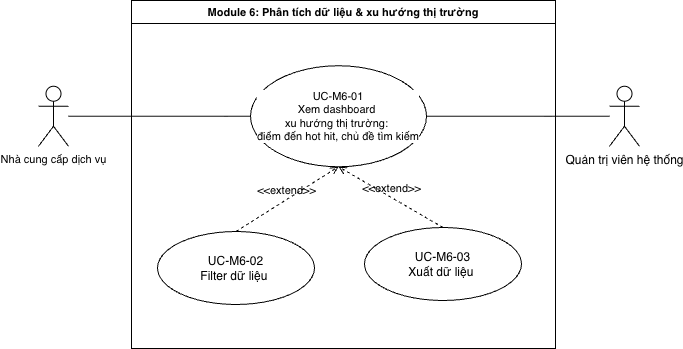
\includegraphics[width=0.9\textwidth]{Images/6. System analysis/6.png}
    \caption{Use case diagram cho Module 6: Phân tích dữ liệu \& xu hướng thị trường}
    \label{fig:use_case_module_6}
\end{figure}
\begin{table}[H]
\caption{Mô tả Use Case: Xem dashboard xu hướng thị trường}
\label{usecase-6-01}
\centering
\renewcommand{\arraystretch}{1.2}
\begin{tabular}{@{}p{4cm} p{11cm}@{}}
\toprule
\textbf{Use case ID}       & UC-M6-01 \\ \midrule
\textbf{Tên Use case}      & Xem dashboard xu hướng thị trường \\ \midrule
\textbf{Các tác nhân}      & Provider, Admin \\ \midrule
\textbf{Mô tả}             & Cung cấp cho Provider, Admin các thông tin về các địa điểm hot được người dùng quan tâm và tìm kiếm.\\ \midrule
\textbf{Trigger}    & Người dùng chọn tab "Phân tích" \space trên thanh điều hướng.\\ \midrule
\textbf{Tiền điều kiện}    & Người dùng đã đăng nhập.\\ \midrule
\textbf{Hậu điều kiện}     & Hệ thống hiển thị biểu đồ và danh sách về xu hướng chung. \\ \midrule
\textbf{Luồng sự kiện chính} & 
\begin{tabular}[t]{@{}p{10.5cm}@{}}
1. Người dùng chọn menu "Phân tích" \space hoặc "Xu hướng thị trường".
2. Hệ thống truy xuất dữ liệu tổng hợp từ log tìm kiếm và đặt chỗ của người dùng.\\
3. Hệ thống hiển thị Dashboard, bao gồm: \\
- Top điểm đến: Biểu đồ cột/tròn các địa điểm được đánh giá cao nhất.\\
- Dịch vụ yêu thích: Tỷ lệ phần trăm các loại tour/khách sạn. \\
4. Người dùng xem tổng quan dữ liệu.    
\end{tabular} \\ \midrule
\textbf{Luồng ngoại lệ} & Nếu hệ thống mất kết nối $\rightarrow$ Hiển thị thông báo "Lỗi kết nối" \\
\bottomrule
\end{tabular}
\end{table}

\begin{table}[H]
\caption{Mô tả Use Case: Filter dữ liệu}
\label{usecase-6-02}
\centering
\renewcommand{\arraystretch}{1.2}
\begin{tabular}{@{}p{4cm} p{11cm}@{}}
\toprule
\textbf{Use case ID}       & UC-M6-02 \\ \midrule
\textbf{Tên Use case}      & Filter dữ liệu\\ \midrule
\textbf{Các tác nhân}      & Provider, Admin \\ \midrule
\textbf{Mô tả}             & Cho phép lọc các chỉ số trên dashboard theo tiêu chí cụ thể.\\ \midrule
\textbf{Tiền điều kiện}    & Người dùng đang xem Dashboard (UC-M6-01).\\ \midrule
\textbf{Hậu điều kiện}     & Dashboard cập nhật hiển thị theo bộ lọc mới. \\ \midrule
\textbf{Luồng sự kiện chính} & 
\begin{tabular}[t]{@{}p{10.5cm}@{}}
1. Trên giao diện Dashboard, Người dùng nhấn vào nút "Bộ lọc".\\
2. Hệ thống hiển thị các tiêu chí lọc: \\
- Khoảng thời gian.\\
- Khu vực.\\
- Danh mục\\
3. Người dùng chọn các giá trị mong muốn và nhấn "Áp dụng".\\
4. Hệ thống truy vấn lại dữ liệu theo tham số mới.\\
5. Hệ thống làm mới các biểu đồ để phản ánh dữ liệu đã lọc.    
\end{tabular} \\ \midrule
\textbf{Luồng ngoại lệ} & 
\begin{tabular}[t]{@{}p{10.5cm}@{}}
\textbf{E1: Không có dữ liệu}\\
Bộ lọc quá chi tiết dẫn đến kết quả rỗng $\rightarrow$ Hệ thống báo "Không tìm thấy dữ liệu phù hợp với bộ lọc này".
\end{tabular} \\
\bottomrule
\end{tabular}
\end{table}

\begin{table}[H]        
\caption{Mô tả Use Case: Xuất dữ liệu}
\label{usecase-6-03}
\centering
\renewcommand{\arraystretch}{1.2}
\begin{tabular}{@{}p{4cm} p{11cm}@{}}
\toprule
\textbf{Use case ID}       & UC-M6-03 \\ \midrule
\textbf{Tên Use case}      & Xuất dữ liệu\\ \midrule
\textbf{Các tác nhân}      & Provider, Admin \\ \midrule
\textbf{Mô tả}             & Tải xuống các số liệu thống kê dưới dạng file (Excel, PDF) để lưu trữ hoặc làm báo cáo.\\ \midrule
\textbf{Tiền điều kiện}    & Người dùng đang xem Dashboard và có thể áp dụng bộ lọc từ UC-M6-02.\\ \midrule
\textbf{Hậu điều kiện}     & File báo cáo được tải xuống. \\ \midrule
\textbf{Luồng sự kiện chính} & 
\begin{tabular}[t]{@{}p{10.5cm}@{}}
1. Người dùng nhấn nút "Xuất báo cáo" \space trên góc màn hình.\\
2. Hệ thống yêu cầu chọn định dạng file (Excel cho dữ liệu thô, PDF cho biểu đồ).\\
3. Người dùng chọn định dạng và nhấn "Tải xuống".\\
4. Hệ thống tổng hợp dữ liệu hiện tại (đang hiển thị trên màn hình).\\
5. Hệ thống tạo file và gửi luồng dữ liệu xuống trình duyệt của Người dùng.\\
6. Người dùng nhận file thành công.    
\end{tabular} \\ 
\bottomrule
\end{tabular}
\end{table}


% --- 8. MODULE 7: GỢI Ý CẢI THIỆN LỊCH TRÌNH ---
\subsubsubsection{Module 7: Gợi ý cải thiện lịch trình}
\begin{figure}[H]
    \centering
    % NOTE: Bổ sung tên file ảnh cho Module 7 (Gợi ý cải thiện)
    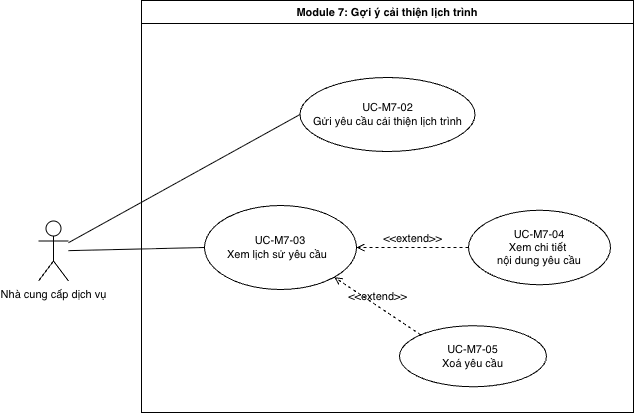
\includegraphics[width=0.9\textwidth]{Images/6. System analysis/7.png}
    \caption{Use case diagram cho Module 7: Gợi ý cải thiện lịch trình}
    \label{fig:use_case_module_7}
\end{figure}
% \begin{longtable}{|p{4cm}|p{11cm}|}
% \caption{Mô tả Use Case: Gửi yêu cầu cải thiện lịch trình}
% \label{usecase-7-02} \\
% \hline
% \endfirsthead
% \caption[]{Mô tả Use Case: Gửi yêu cầu cải thiện lịch trình} \\
% \hline
% \endhead
% \textbf{Use case ID}       & UC-M7-02 \\ \hline
% \textbf{Tên Use case}      & Gửi yêu cầu cải thiện lịch trình \\ \hline
% \textbf{Các tác nhân}      & Provider \\ \hline
% \textbf{Mô tả}             & Provider cung cấp thông tin lịch trình hiện tại và các tiêu chí mong muốn. Hệ thống AI đọc dữ liệu trực tiếp, phân tích, chỉ ra điểm yếu và tự động tái cấu trúc để tạo ra một phiên bản lịch trình mới tối ưu hơn.\\ \hline
% \textbf{Trigger}    & Người dùng đã đăng nhập vào hệ thống.\\ \hline
% \textbf{Tiền điều kiện}    & Người dùng đã đăng nhập.\\ \hline
% \textbf{Hậu điều kiện}     & Một phiên bản lịch trình mới được tạo ra và lưu vào danh sách đề xuất. \\ \hline
% \textbf{Luồng sự kiện chính} & 
% \begin{tabular}[t]{@{}p{10.5cm}@{}}
% 1. Provider truy cập tab "Gợi ý".\\
% 2. Provider nhấn "Tạo yêu cầu mới".\\
% 3. Provider nhập thông tin lịch trình hiện tại và các tiêu chí mong muốn\\
% 4. Provider nhấn nút "Phân tích \& Tối ưu hóa".\\
% 5. Hệ thống gửi dữ liệu đến Module AI để xử lý.\\
% 6. Hệ thống trả về kết quả gồm 2 phần:\\
% - Phần phân tích: Báo cáo điểm mạnh/điểm yếu của lịch trình cũ.\\
% - Phần giải pháp: Hiển thị lịch trình mới đã được sắp xếp lại, thay thế các điểm chưa hợp lý bằng các gợi ý tốt hơn.\\
% 7. Provider xem xét và có thể chọn "Lưu bản nháp" \space hoặc "Áp dụng ngay".
% \end{tabular} \\ \hline
% \textbf{Luồng rẽ nhánh} &
% \begin{tabular}[t]{@{}p{10.5cm}@{}}
% \textbf{A1: So sánh trực quan}\\
% 1. Tại bước 6, Provider chọn chế độ "So sánh".\\
% 2. Hệ thống hiển thị giao diện chia đôi màn hình: bên trái là lịch trình gốc, bên phải là lịch trình gợi ý.\\
% 3. Các thay đổi được làm nổi bật bằng màu khác biệt để dễ nhận biết.\\
% \textbf{A2: Chỉnh sửa lại gợi ý}\\
% 1. Provider thấy gợi ý của AI tốt nhưng muốn sửa lại một điểm nhỏ.\\
% 2. Provider nhấn "Chỉnh sửa kết quả" \space trực tiếp trên giao diện gợi ý.\\
% 3. Hệ thống cho phép sửa đổi thủ công trước khi lưu.
% \end{tabular} \\ \hline
% \textbf{Luồng ngoại lệ} &
% \begin{tabular}[t]{@{}p{10.5cm}@{}}
% \textbf{E1: Không tìm thấy giải pháp tối ưu}\\
% AI nhận thấy các ràng buộc của Provider mâu thuẫn. Hệ thống thông báo: "Không thể tạo lịch trình đáp ứng đủ tất cả tiêu chí."
% \end{tabular} \\
% \hline
% \end{longtable}

% \begin{longtable}{|p{4cm}|p{11cm}|}
% \caption{Mô tả Use Case: Xem lịch sử yêu cầu}
% \label{usecase-7-03} \\
% \hline
% \endfirsthead
% \caption[]{Mô tả Use Case: Xem lịch sử yêu cầu} \\
% \hline
% \endhead
% \textbf{Use case ID}       & UC-M7-03 \\ \hline
% \textbf{Tên Use case}      & Xem lịch sử yêu cầu \\ \hline
% \textbf{Các tác nhân}      & Provider \\ \hline
% \textbf{Mô tả}             & Xem lại danh sách các lần đã nhờ AI tư vấn trước đó.\\ \hline
% \textbf{Tiền điều kiện}    & Provider đã đăng nhập.\\ \hline
% \textbf{Hậu điều kiện}     & Danh sách lịch sử yêu cầu được hiển thị. \\ \hline
% \textbf{Luồng sự kiện chính} & 
% \begin{tabular}[t]{@{}p{10.5cm}@{}}
% 1. Provider chọn mục "Lịch sử tư vấn".\\
% 2. Hệ thống lấy danh sách các yêu cầu thuộc về Provider này.\\
% 3. Hệ thống hiển thị danh sách các yêu cầu.\\
% 4. Provider có thể thực hiện các hành động mở rộng (Xem chi tiết, Xóa) từ danh sách này.\\
% \end{tabular} \\
% \hline
% \end{longtable}

% % \begin{longtable}{|p{4cm}|p{11cm}|}
% % \caption{Mô tả Use Case: Xem chi tiết nội dung yêu cầu}
% % \label{usecase-7-04} \\
% % \hline
% % \endfirsthead
% % \caption[]{Mô tả Use Case: Xem chi tiết nội dung yêu cầu} \\
% % \hline
% % \endhead
% % \textbf{Use case ID}       & UC-M7-04 \\ \hline
% % \textbf{Tên Use case}      & Xem chi tiết nội dung yêu cầu \\ \hline
% % \textbf{Các tác nhân}      & Provider \\ \hline
% % \textbf{Mô tả}             & Xem lại toàn bộ nội dung input và output của một yêu cầu trong quá khứ.\\ \hline
% % \textbf{Tiền điều kiện}    & Provider đang ở màn hình lịch sử yêu cầu (UC-M7-03).\\ \hline
% % \textbf{Hậu điều kiện}     & Nội dung chi tiết được hiển thị. \\ \hline
% % \textbf{Luồng sự kiện chính} & 
% % \begin{tabular}[t]{@{}p{10.5cm}@{}}
% % 1. Từ danh sách lịch sử, Provider nhấn vào một dòng yêu cầu cụ thể.\\
% % 2. Hệ thống tải dữ liệu chi tiết của phiên tư vấn đó.\\
% % 3. Hệ thống hiển thị giao diện chia đôi hoặc trên dưới:\\
% % - Yêu cầu gốc: Lộ trình và mục tiêu Provider đã nhập.\\
% % - Kết quả AI: Các gợi ý đã được tạo ra lúc đó.\\
% % 4. Provider có thể tham khảo lại hoặc sao chép nội dung gợi ý.
% % \end{tabular} \\
% % \hline
% % \end{longtable}

% % \begin{longtable}{|p{4cm}|p{11cm}|}
% % \caption{Mô tả Use Case: Xóa yêu cầu}
% % \label{usecase-7-05} \\
% % \hline
% % \endfirsthead
% % \caption[]{Mô tả Use Case: Xóa yêu cầu} \\
% % \hline
% % \endhead
% % \textbf{Use case ID}       & UC-M7-04 \\ \hline
% % \textbf{Tên Use case}      & Xóa yêu cầu \\ \hline
% % \textbf{Các tác nhân}      & Provider \\ \hline
% % \textbf{Mô tả}             & Xóa bỏ một bản ghi lịch sử tư vấn không còn cần thiết.\\ \hline
% % \textbf{Tiền điều kiện}    & Provider đang ở màn hình lịch sử yêu cầu (UC-M7-03).\\ \hline
% % \textbf{Hậu điều kiện}     & Bản ghi bị xóa khỏi CSDL. \\ \hline
% % \textbf{Luồng sự kiện chính} & 
% % \begin{tabular}[t]{@{}p{10.5cm}@{}}
% % 1. Tại dòng yêu cầu muốn xóa, Provider nhấn nút "Xóa".\\
% % 2. Hệ thống hiển thị popup xác nhận: "Bạn có chắc chắn muốn xóa lịch sử tư vấn này không?".\\
% % 3. Provider nhấn "Xác nhận xóa".\\
% % 4. Hệ thống thực hiện xóa bản ghi trong CSDL.\\
% % 5. Hệ thống tải lại danh sách lịch sử mới và thông báo "Đã xóa thành công".
% % \end{tabular} \\ \hline
% % \textbf{Luồng rẽ nhánh} &
% % \begin{tabular}[t]{@{}p{10.5cm}@{}}
% % \textbf{A1: Hủy xóa:}\\
% % Tại bước 3, Provider nhấn "Hủy" $\rightarrow$ Popup đóng lại, không có gì thay đổi.
% % \end{tabular} \\
% % \hline
% % \end{longtable}



% --- 9. MODULE 8: QUẢN TRỊ NGƯỜI DÙNG ---
\subsubsubsection{Module 8: Quản trị người dùng}
\begin{figure}[H]
    \centering
    % NOTE: Bổ sung tên file ảnh cho Module 8 (Quản trị người dùng)
    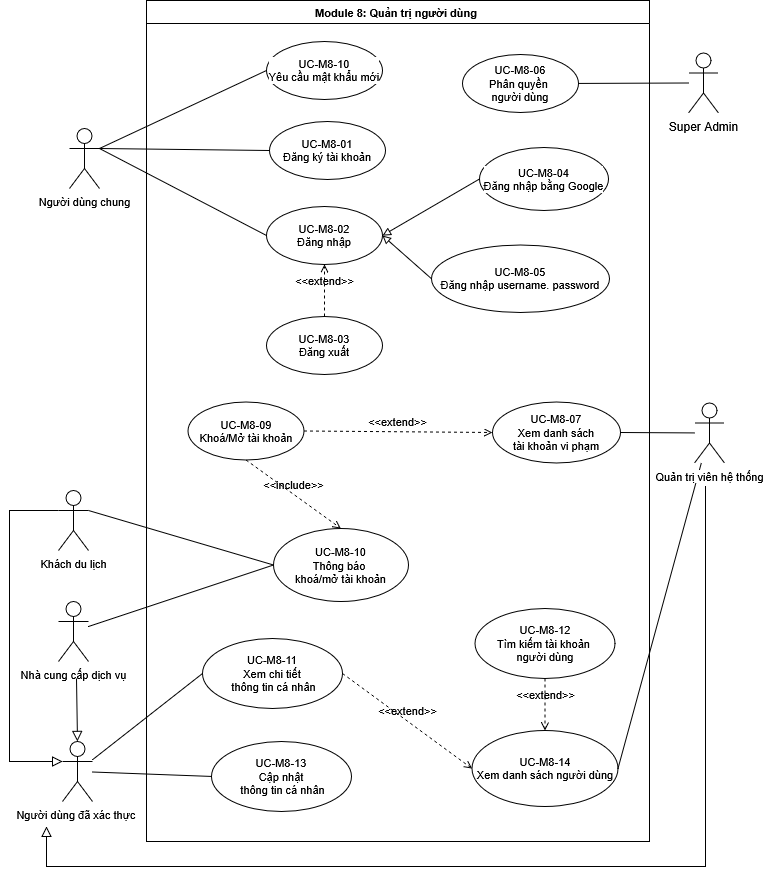
\includegraphics[width=0.9\textwidth]{Images/6. System analysis/8.png}
    \caption{Use case diagram cho Module 8: Quản trị người dùng}
    \label{fig:use_case_module_8}
\end{figure}
% \begin{longtable}{|p{4cm}|p{11cm}|}
% \caption{Mô tả Use Case: Đăng ký tài khoản}
% \label{usecase-8-01} \\
% \hline
% \endfirsthead
% \caption[]{Mô tả Use Case: Đăng ký tài khoản} \\
% \hline
% \endhead
% \textbf{Use case ID}       & UC-M8-01 \\ \hline
% \textbf{Tên Use case}      & Đăng ký tài khoản \\ \hline
% \textbf{Các tác nhân}      & Guest \\ \hline
% \textbf{Mô tả}             & Tạo tài khoản mới cho người dùng.\\ \hline
% \textbf{Tiền điều kiện}    & Người dùng chưa đăng nhập\\ \hline
% \textbf{Hậu điều kiện}     & Tài khoản mới được thêm vào hệ thống \\ \hline
% \textbf{Trigger}    & Người dùng bấm "Đăng ký". \\ \hline
% \textbf{Luồng sự kiện chính} & 
% \begin{tabular}[t]{@{}p{10.5cm}@{}}
% 1. Người dùng nhấn nút "Đăng ký".\\
% 2. Hệ thống hiển thị trang có form đăng ký tài khoản.\\
% 3. Người dùng nhập thông tin để đăng ký tài khoản.\\
% 4. Hệ thống kiểm tra định dạng và trùng lặp.\\
% 5. Hệ thống tạo tài khoản.\\
% 6. Hệ thống chuyển sang trang đăng nhập.
% \end{tabular} \\ \hline
% \textbf{Luồng ngoại lệ} &
% \begin{tabular}[t]{@{}p{10.5cm}@{}}
% \textbf{E1: Lỗi từ người dùng}\\
% Báo lỗi "Thông tin không hợp lệ". \\
% \textbf{E2: Lỗi từ hệ thống}\\
% Báo lỗi "Lỗi hệ thống". 
% \end{tabular} \\
% \hline
% \end{longtable}

% \begin{longtable}{|p{4cm}|p{11cm}|}
% \caption{Mô tả Use Case: Đăng nhập bằng tài khoản Google}
% \label{usecase-8-03} \\
% \hline
% \endfirsthead
% \caption[]{Mô tả Use Case: Đăng nhập bằng tài khoản Google} \\
% \hline
% \endhead
% \textbf{Use case ID}       & UC-M8-02 \\ \hline
% \textbf{Tên Use case}      & Đăng nhập bằng tài khoản Google \\ \hline
% \textbf{Các tác nhân}      & Guest \\ \hline
% \textbf{Mô tả}             & Cho phép người dùng đăng nhập vào hệ thống qua tài khoản Google. \\ \hline
% \textbf{Tiền điều kiện}    & Trình duyệt không bị chặn cookie cần thiết. \\ \hline
% \textbf{Hậu điều kiện}     & Người dùng đăng nhập thành công vào hệ thống.\\ \hline
% \textbf{Trigger}    & Người dùng bấm "Đăng nhập bằng Google". \\ \hline
% \textbf{Luồng sự kiện chính} & 
% \begin{tabular}[t]{@{}p{10.5cm}@{}}
% 1. Chọn phương thức đăng nhập bằng Google . 
% 2. Hệ thống điều hướng sang trang đăng nhập với Google
% 3. Người dùng chọn account muốn đăng nhập
% 4. Hệ thống xác thực
% 5. Hệ thống tạo session/JWT và chuyển vào ứng dụng.
% 6. Hệ thống chuyển sang trang chính.
% \end{tabular} \\ \hline
% \textbf{Luồng rẽ nhánh} &
% \begin{tabular}[t]{@{}p{10.5cm}@{}}
% \textbf{A1: Tài khoản google đã tồn tại trong hệ thống}\\
% 1. Người dùng đăng nhập thành công.\\
% \textbf{A2: Tài khoản google không tồn tại trong hệ thống}\\
% 1. Tài khoản mới được tạo và lưu vào hệ thống.\\
% 2. Người dùng đăng nhập thành công.\\
% \end{tabular} \\
% \hline
% \end{longtable}

% \begin{longtable}{|p{4cm}|p{11cm}|}
% \caption{Mô tả Use Case: Đăng nhập bằng username, password}
% \label{usecase-8-04} \\
% \hline
% \endfirsthead
% \caption[]{Mô tả Use Case: Đăng nhập bằng username, password} \\
% \hline
% \endhead
% \textbf{Use case ID}       & UC-M8-03 \\ \hline
% \textbf{Tên Use case}      & Đăng nhập bằng username, password \\ \hline
% \textbf{Các tác nhân}      & Guest \\ \hline
% \textbf{Mô tả}             & Cho phép người dùng đăng nhập vào hệ thống qua tài khoản username và password. \\ \hline
% \textbf{Tiền điều kiện}    & Người dùng đã có tài khoản trong hệ thống. \\ \hline
% \textbf{Hậu điều kiện}     & Người dùng đăng nhập thành công vào hệ thống.\\ \hline
% \textbf{Trigger}    & Người dùng bấm "Đăng nhập bằng username, password". \\ \hline
% \textbf{Luồng sự kiện chính} & 
% \begin{tabular}[t]{@{}p{10.5cm}@{}}
% 1. Chọn phương thức đăng nhập bằng username, password . 
% 2. Hệ thống hiển thị form đăng nhập
% 3. Người dùng điền username và password
% 4. Hệ thống xác thực tài khoản
% 5. Hệ thống tạo session/JWT và chuyển vào ứng dụng.
% 6. Hệ thống chuyển sang trang chính.
% \end{tabular} \\ \hline
% \textbf{Luồng ngoại lệ} &
% \begin{tabular}[t]{@{}p{10.5cm}@{}}
% \textbf{E1: Lỗi từ người dùng}\\
% Báo lỗi "Tài khoản hoặc mật khẩu không đúng". \\
% \textbf{E2: Lỗi từ hệ thống}\\
% Báo lỗi "Lỗi hệ thống". 
% \end{tabular} \\
% \hline
% \end{longtable}

% \begin{longtable}{|p{4cm}|p{11cm}|}
% \caption{Mô tả Use Case: Đăng xuất}
% \label{usecase-8-05} \\
% \hline
% \endfirsthead
% \caption[]{Mô tả Use Case: Đăng xuất} \\
% \hline
% \endhead
% \textbf{Use case ID}       & UC-M8-05 \\ \hline
% \textbf{Tên Use case}      & Đăng xuất \\ \hline
% \textbf{Các tác nhân}      & Traveler, Provider, Admin \\ \hline
% \textbf{Mô tả}             & Cho phép người dùng đăng xuất khỏi hệ thống. \\ \hline
% \textbf{Tiền điều kiện}    & Người dùng đã đăng nhập vào hệ thống. \\ \hline
% \textbf{Hậu điều kiện}     & Người dùng đăng xuất khỏi hệ thống thành công. \\ \hline
% \textbf{Trigger}    & Người dùng bấm "Đăng xuất". \\ \hline
% \textbf{Luồng sự kiện chính} & 
% \begin{tabular}[t]{@{}p{10.5cm}@{}}
% 1. Người dùng bấm "Đăng xuất".
% 2. Hệ thống hủy session, clear cookie.
% 3. Điều hướng về trang chính.
% \end{tabular} \\
% \hline
% \end{longtable}

\begin{longtable}{|p{4cm}|p{11cm}|}
\caption{Mô tả Use Case: Xem chi tiết thông tin cá nhân}
\label{usecase-8-11} \\
\hline
\endfirsthead
\caption[]{Mô tả Use Case: Xem chi tiết thông tin cá nhân} \\
\hline
\endhead
\textbf{Use case ID}       & UC-M8-11 \\ \hline
\textbf{Tên Use case}      & Xem chi tiết thông tin cá nhân \\ \hline
\textbf{Các tác nhân}      & Traveler, Provider, Admin \\ \hline
\textbf{Mô tả}             & Xem thông tin hồ sơ cá nhân. \\ \hline
\textbf{Tiền điều kiện}    & Người dùng đã đăng nhập vào hệ thống. \\ \hline
\textbf{Hậu điều kiện}     & Hiển thị thông tin hồ sơ cá nhân. \\ \hline
\textbf{Trigger}    & Mở trang "Thông tin của tôi". \\ \hline
\textbf{Luồng sự kiện chính} & 
\begin{tabular}[t]{@{}p{10.5cm}@{}}
1. Người dùng truy cập trang "Thông tin của tôi. 
2. Hệ thống hiển thị thông tin của người dùng. \\
\end{tabular} \\
\hline
\end{longtable}

\begin{longtable}{|p{4cm}|p{11cm}|}
\caption{Mô tả Use Case: Xem danh sách người dùng}
\label{usecase-8-14} \\
\hline
\endfirsthead
\caption[]{Mô tả Use Case: Xem danh sách người dùng} \\
\hline
\endhead
\textbf{Use case ID}       & UC-M8-14 \\ \hline
\textbf{Tên Use case}      & Xem danh sách người dùng \\ \hline
\textbf{Các tác nhân}      & Admin \\ \hline
\textbf{Mô tả}             & Xem danh sách toàn bộ người dùng.\\ \hline
\textbf{Tiền điều kiện}    & Admin đã đăng nhập vào hệ thống. \\ \hline
\textbf{Hậu điều kiện}     & Hiển thị danh sách toàn bộ người dùng. \\ \hline
\textbf{Luồng sự kiện chính} & 
\begin{tabular}[t]{@{}p{10.5cm}@{}}
1. Admin truy cập trang "Danh sách người dùng". \\
2. Hệ thống hiển thị danh sách người dùng. \\
3. Admin có thể chọn lọc theo vai trò, trạng thái, thời điểm tạo, sắp xếp.
\end{tabular} \\
\hline
\end{longtable}

\begin{longtable}{|p{4cm}|p{11cm}|}
\caption{Mô tả Use Case: Xem danh sách tài khoản vi phạm}
\label{usecase-8-07} \\
\hline
\endfirsthead
\caption[]{Mô tả Use Case: Xem danh sách tài khoản vi phạm} \\
\hline
\endhead
\textbf{Use case ID}       & UC-M8-07 \\ \hline
\textbf{Tên Use case}      & Xem danh sách tài khoản vi phạm \\ \hline
\textbf{Các tác nhân}      & Admin \\ \hline
\textbf{Mô tả}             & Xem danh sách các tài khoản bị báo cáo vi phạm quy định.\\ \hline
\textbf{Tiền điều kiện}    & Admin đã đăng nhập vào hệ thống. \\ \hline
\textbf{Hậu điều kiện}     & Hiển thị danh sách tài khoản vi phạm \\ \hline
\textbf{Luồng sự kiện chính} & 
\begin{tabular}[t]{@{}p{10.5cm}@{}}
1. Admin truy cập trang "Tài khoản vi phạm". \\
2. Hệ thống hiển thị danh sách các tài khoản vi phạm. \\
3. (Tùy chọn) Lọc theo mức độ, thời gian, loại vi phạm. \\
4. Chọn một tài khoản để xem chi tiết hoặc thực hiện thao tác (khóa/mở tài khoản). \\
\end{tabular} \\
\hline
\end{longtable}

\begin{longtable}{|p{4cm}|p{11cm}|}
\caption{Mô tả Use Case: Khóa/Mở tài khoản}
\label{usecase-8-07} \\
\hline
\endfirsthead
\caption[]{Mô tả Use Case: Khóa/Mở tài khoản} \\
\hline
\endhead
\textbf{Use case ID}       & UC-M8-07 \\ \hline
\textbf{Tên Use case}      & Khóa/Mở tài khoản \\ \hline
\textbf{Các tác nhân}      & Admin \\ \hline
\textbf{Mô tả}             & Khóa/Mở tài khoản.\\ \hline
\textbf{Tiền điều kiện}    & Xác định được tài khoản mục tiêu; trạng thái hiện tại cho phép thao tác khóa/mở tài khoản.\\ \hline
\textbf{Hậu điều kiện}     & Trạng thái tài khoản được cập nhật thành công. Thông báo cho người dùng. \\ \hline
\textbf{Luồng sự kiện chính} & 
\begin{tabular}[t]{@{}p{10.5cm}@{}}
1. Admin chọn tài khoản và hành động khóa/mở tài khoản.\\
2. Nhập lý do.\\
3. Xác nhận thao tác.\\
4. Hệ thống cập nhật trạng thái.\\
5. Thông báo cho người dùng.
\end{tabular} \\
\hline
\end{longtable}



% --- 10. MODULE 9: QUẢN TRỊ HỆ THỐNG ---
\subsubsubsection{Module 9: Quản trị hệ thống}
\begin{figure}[H]
    \centering
    % NOTE: Bổ sung tên file ảnh cho Module 9 (Quản trị hệ thống)
    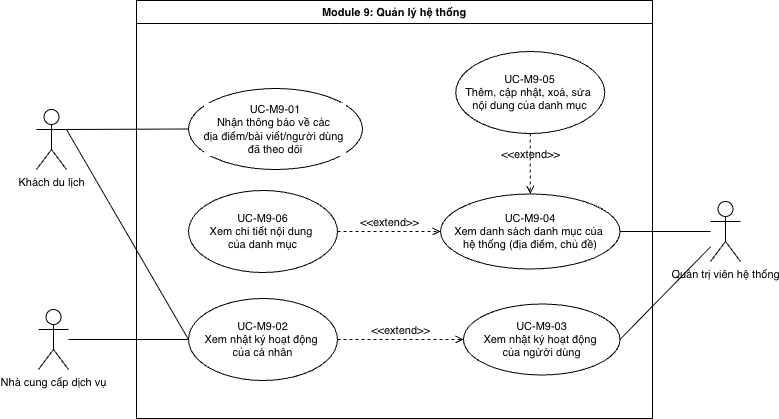
\includegraphics[width=0.9\textwidth]{Images/6. System analysis/9.png}
    \caption{Use case diagram cho Module 9: Quản trị hệ thống}
    \label{fig:use_case_module_9}
\end{figure}
\begin{longtable}{@{}p{4cm} p{11cm}@{}}
\caption{Mô tả Use Case: Nhận thông báo từ các nội dung theo dõi}
\label{usecase-9-01} \\
\toprule
\textbf{Use case ID}       & UC-M9-01 \\ \midrule
\textbf{Tên Use case}      & Nhận thông báo về các địa điểm, bài viết người dùng đã theo dõi \\ \midrule
\textbf{Các tác nhân}      & Traveler \\ \midrule
\textbf{Mô tả}             & Nhận thông báo khi có cập nhật mới từ các mục mà người dùng đã theo dõi.\\ \midrule
\textbf{Tiền điều kiện}    &
\begin{tabular}[t]{@{}p{10.5cm}@{}}
    1. Người dùng đã đăng nhập vào hệ thống.\\
    2. Người dùng đã theo dõi ít nhất một đối tượng.
    \end{tabular} \\ \midrule
\textbf{Hậu điều kiện}     & Hiển thị danh sách thông báo về các nội dung người dùng đã theo dõi. \\ \midrule
\textbf{Luồng sự kiện chính} & 
\begin{tabular}[t]{@{}p{10.5cm}@{}}
1. Hệ thống kiểm tra định kỳ hoặc nhận sự kiện mới (bài viết mới, địa điểm cập nhật, người dùng đăng bài).\\
2. Hệ thống tạo nội dung thông báo tương ứng.\\
3. Hệ thống gửi thông báo đến người dùng.\\
4. Người dùng xem thông báo trong trung tâm thông báo.
\end{tabular} \\
\bottomrule
\end{longtable}

\begin{longtable}{@{}p{4cm} p{11cm}@{}}
\caption{Mô tả Use Case: Xem nhật ký hoạt động của cá nhân}
\label{usecase-9-02} \\
\toprule
\textbf{Use case ID}       & UC-M9-02 \\ \midrule
\textbf{Tên Use case}      & Xem nhật ký hoạt động của cá nhân \\ \midrule
\textbf{Các tác nhân}      & Traveler, Provider \\ \midrule
\textbf{Mô tả}             & Người dùng xem lại lịch sử hoạt động của cá nhân.\\ \midrule
\textbf{Tiền điều kiện}    & Người dùng đã đăng nhập vào hệ thống. \\ \midrule
\textbf{Hậu điều kiện}     & Hiển thị danh sách hoạt động của người dùng. \\ \midrule
\textbf{Luồng sự kiện chính} & 
\begin{tabular}[t]{@{}p{10.5cm}@{}}
1. Người dùng mở mục "Nhật ký hoạt động của tôi".\\
2. Hệ thống hiển thị danh sách hoạt động gần nhất theo ngày.\\
3. Người dùng có thể lọc theo loại khoảng thời gian.
\end{tabular} \\
\bottomrule
\end{longtable}

\begin{longtable}{@{}p{4cm} p{11cm}@{}}
\caption{Mô tả Use Case: Xem nhật ký hoạt động của người dùng}
\label{usecase-9-03} \\
\toprule
\textbf{Use case ID}       & UC-M9-03 \\ \midrule
\textbf{Tên Use case}      & Xem nhật ký hoạt động của người dùng \\ \midrule
\textbf{Các tác nhân}      & Admin \\ \midrule
\textbf{Mô tả}             & Quản trị viên xem lịch sử hoạt động của người dùng trong hệ thống.\\ \midrule
\textbf{Tiền điều kiện}    & Quản trị viên đã đăng nhập vào hệ thống. \\ \midrule
\textbf{Hậu điều kiện}     & Hiển thị danh sách hoạt động của người dùng trong hệ thống. \\ \midrule
\textbf{Luồng sự kiện chính} & 
\begin{tabular}[t]{@{}p{10.5cm}@{}}
1. Mở trang "Nhật ký hoạt động người dùng".\\
2. Nhập tiêu chí lọc.\\
3. Hệ thống truy xuất và hiển thị kết quả.\\
4. Quản trị viên có thể xem chi tiết hoạt động của người dùng.
\end{tabular} \\
\bottomrule
\end{longtable}

\begin{longtable}{@{}p{4cm} p{11cm}@{}}
\caption{Mô tả Use Case: Xem danh sách danh mục của hệ thống (Địa điểm, chủ đề)}
\label{usecase-9-04} \\
\toprule
\textbf{Use case ID}       & UC-M9-04 \\ \midrule
\textbf{Tên Use case}      & Xem danh sách danh mục của hệ thống (Địa điểm, chủ đề) \\ \midrule
\textbf{Các tác nhân}      & Admin \\ \midrule
\textbf{Mô tả}             & Quản trị viên xem danh sách danh mục của hệ thống (Địa điểm, chủ đề).\\ \midrule
\textbf{Tiền điều kiện}    & Quản trị viên đã đăng nhập vào hệ thống. \\ \midrule
\textbf{Hậu điều kiện}     & Hiển thị danh sách danh mục của hệ thống (Địa điểm, chủ đề). \\ \midrule
\textbf{Luồng sự kiện chính} & 
\begin{tabular}[t]{@{}p{10.5cm}@{}}
1. Mở phần "Danh mục hệ thống".\\
2. Hệ thống hiển thị danh sách các nội dung theo từng danh mục.\\
3. Có thể lọc hoặc sắp xếp danh sách.\\
4. Chọn danh mục để xem chi tiết hoặc chuyển sang thao tác khác (thêm, xóa, sửa).
\end{tabular} \\
\bottomrule
\end{longtable}

\begin{longtable}{@{}p{4cm} p{11cm}@{}}
\caption{Mô tả Use Case: Thêm, xóa, sửa nội dung của danh mục}
\label{usecase-9-05} \\
\toprule
\textbf{Use case ID}       & UC-M9-05 \\ \midrule
\textbf{Tên Use case}      & Xem danh sách danh mục của hệ thống (Địa điểm, chủ đề) \\ \midrule
\textbf{Các tác nhân}      & Admin \\ \midrule
\textbf{Mô tả}             & Quản trị viên xem danh sách danh mục của hệ thống (Địa điểm, chủ đề).\\ \midrule
\textbf{Tiền điều kiện}    & Quản trị viên đã đăng nhập vào hệ thống. \\ \midrule
\textbf{Hậu điều kiện}     & Hiển thị danh sách danh mục của hệ thống (Địa điểm, chủ đề). \\ \midrule
\textbf{Luồng sự kiện chính} & 
\begin{tabular}[t]{@{}p{10.5cm}@{}}
1. Quản trị viên chọn thao tác: thêm, sửa, hoặc xóa nội dung theo từng danh mục.\\
2. Hệ thống hiển thị form nhập thông tin hoặc xác nhận thao tác.\\
3. Quản trị viên nhập dữ liệu hợp lệ (tên, mô tả, hình ảnh, trạng thái…).\\
4. Hệ thống kiểm tra dữ liệu và lưu thay đổi.\\
5. Thông báo kết quả thao tác.    
\end{tabular} \\
\bottomrule
\end{longtable}

\begin{longtable}{@{}p{4cm} p{11cm}@{}}
\caption{Mô tả Use Case: Xem chi tiết nội dung của danh mục}
\label{usecase-9-06} \\
\toprule
\textbf{Use case ID}       & UC-M9-06 \\ \midrule
\textbf{Tên Use case}      & Xem chi tiết nội dung của danh mục \\ \midrule
\textbf{Các tác nhân}      & Traveler, Provider, Admin \\ \midrule
\textbf{Mô tả}             & Xem thông tin chi tiết về một danh mục cụ thể. \\ \midrule
\textbf{Tiền điều kiện}    & Danh mục hợp lệ và hiển thị công khai. \\ \midrule
\textbf{Hậu điều kiện}     & Hiển thị thông tin chi tiết về danh mục. \\ \midrule
\textbf{Luồng sự kiện chính} & 
\begin{tabular}[t]{@{}p{10.5cm}@{}}
1. Người dùng chọn nội dung muốn xem từ danh sách hiển thị.\\
2. Hệ thống hiển thị chi tiết.
\end{tabular} \\
\bottomrule
\end{longtable}

